\documentclass[a4paper,12pt]{article}

%------------------------- packages -------------------------%
\usepackage[utf8]{inputenc}
\usepackage[T5]{fontenc}
\usepackage[vietnamese,english]{babel}
\usepackage[unicode,hidelinks]{hyperref}
\usepackage{graphicx}
\graphicspath{{../pics/}{./pics/}{pics/}}
\usepackage{tikz}
\usetikzlibrary{calc, positioning, arrows.meta, shapes.geometric, automata, backgrounds, shadows}
\usepackage{tikz-timing} % Required for waveform diagram
\usepackage{amsmath}
\usepackage{geometry}
\usepackage{titlesec}
\usepackage{array}
\usepackage{fancyhdr}
\usepackage{lastpage}
\usepackage{setspace}
\usepackage{tabularx}
\usepackage{multirow}
\usepackage{enumitem}
\usepackage{adjustbox}
\usepackage{amsfonts,amssymb}
\DeclareUnicodeCharacter{2713}{\ensuremath{\checkmark}}
\usepackage{float}
\usepackage{listings}
\usepackage{tcolorbox}
\usepackage{caption}
\usepackage{inconsolata}
\usepackage{tocloft} 
\usepackage[normalem]{ulem}
\usepackage[svgnames]{xcolor}

%------------------------- custom colors -------------------------%
\definecolor{vgreen}{rgb}{0,0.6,0}
\definecolor{vgray}{rgb}{0.5,0.5,0.5}
\definecolor{vpurple}{rgb}{0.58,0,0.82}
\definecolor{vback}{rgb}{0.96,0.96,0.94}
\definecolor{cppblue}{rgb}{0.13,0.13,1}
\definecolor{cppgreen}{rgb}{0,0.5,0}
\definecolor{cppred}{rgb}{0.9,0,0}
\definecolor{outback}{rgb}{0.1,0.1,0.1}
\definecolor{outtext}{rgb}{0.2,0.9,0.2}

%------------------------- lstlisting styles -------------------------%
\lstdefinestyle{VerilogStyle}{
    backgroundcolor=\color{vback},   
    commentstyle=\color{vgreen}\itshape,
    keywordstyle=\color{blue}\bfseries,
    numberstyle=\tiny\color{vgray},
    stringstyle=\color{vpurple},
    basicstyle=\ttfamily\footnotesize,
    breakatwhitespace=false,         
    breaklines=true,                 
    captionpos=b,                    
    keepspaces=true,                 
    numbers=left,                    
    numbersep=10pt,                  
    showspaces=false,                
    showstringspaces=false,
    showtabs=false,                  
    tabsize=4,
    language=Verilog,
    frame=shadowbox,
    rulesepcolor=\color{SteelBlue},
    xleftmargin=15pt,
    xrightmargin=5pt
}

\lstdefinestyle{CppStyle}{
    backgroundcolor=\color{vback},   
    commentstyle=\color{cppgreen}\itshape,
    keywordstyle=\color{cppblue}\bfseries,
    numberstyle=\tiny\color{vgray},
    stringstyle=\color{cppred},
    basicstyle=\ttfamily\footnotesize,
    breakatwhitespace=false,         
    breaklines=true,                 
    captionpos=b,                    
    keepspaces=true,                 
    numbers=left,                    
    numbersep=10pt,                  
    showspaces=false,                
    showstringspaces=false,
    showtabs=false,                  
    tabsize=4,
    language=C++,
    frame=shadowbox,
    rulesepcolor=\color{SteelBlue},
    xleftmargin=15pt,
    xrightmargin=5pt
}

\lstdefinestyle{OutputStyle}{
    backgroundcolor=\color{outback},   
    basicstyle=\ttfamily\footnotesize\color{outtext},
    breaklines=true,                 
    captionpos=b,                    
    keepspaces=true,                 
    numbers=none,                    
    showspaces=false,                
    showstringspaces=false,
    showtabs=false,                  
    tabsize=4,
    frame=single,
    rulecolor=\color{black},
    xleftmargin=5pt,
    xrightmargin=5pt
}

\lstset{
    backgroundcolor=\color{vback},
    basicstyle=\ttfamily\small,
    breakatwhitespace=false,
    breaklines=true,
    captionpos=b,
    columns=fullflexible,
    keepspaces=true,
    numbers=left,
    numbersep=8pt,
    numberstyle=\tiny\color{vgray},
    frame=single,
    framesep=5pt,
    keywordstyle=\color{cppblue}\bfseries,
    commentstyle=\color{cppgreen}\itshape,
    stringstyle=\color{vpurple},
    framerule=0.4pt,
    rulecolor=\color{SteelBlue},
    showstringspaces=false,
    tabsize=4,
    xleftmargin=1.5em,
    xrightmargin=0.5em,
    framexleftmargin=1.2em,
    aboveskip=1em,
    belowskip=1em
}

\newenvironment{fitdiagram}
    {\begin{adjustbox}{max width=\linewidth,max totalheight=0.72\textheight}}
    {\end{adjustbox}}

\setlength{\tabcolsep}{4pt}
\renewcommand{\arraystretch}{1.2}
\captionsetup{font=small,labelfont=bf,skip=6pt}

\tcbset{
    colback=AliceBlue,        
    colframe=SteelBlue,       
    coltitle=MidnightBlue,    
    coltext=DarkSlateGray,    
    fonttitle=\bfseries       
}

%------------------------- set up -------------------------%
\geometry{
    left=2cm,
    right=2cm,
    top=2.5cm,
    bottom=2.5cm,
}

%------------------------- header & footer -------------------------%
\renewcommand{\headrulewidth}{0.5pt}
\renewcommand{\footrulewidth}{0.5pt}
\setlength{\headheight}{35pt}
\pagestyle{fancy}

\fancyhead{}    
\fancyhead[L]{
    \begin{tabular}{ll}
        \begin{picture}(10,10)
            \put(0,-7){
\includegraphics[width=8mm]{hcmut.png}}
        \end{picture}&
        \begin{tabular}{l}
            {\ttfamily Trường Đại học Bách Khoa Tp. Hồ Chí Minh} \\
            {\ttfamily Khoa Khoa học và Kỹ thuật Máy tính} \\
        \end{tabular}   
    \end{tabular}
}

\fancyfoot{}    
\fancyfoot[L]{\footnotesize {\ttfamily CO3069 - Báo cáo Bài tập lớn: Phát triển ứng dụng mật mã và truyền thông bảo mật}}
\fancyfoot[R]{\footnotesize {\ttfamily Trang {\thepage}/\pageref{LastPage}}}

%------------------------- title format settings -------------------------%
\titleformat{\section}
  {\normalfont\Large\bfseries\color{MidnightBlue}}{\thesection}{1em}{}
\titleformat{\subsection}
  {\normalfont\large\bfseries\color{SteelBlue}}{\thesubsection}{1em}{}

% Multi-layered Blue Border Definition
\newcommand{\coverpageborder}{
    \begin{tikzpicture}[remember picture,overlay,inner sep=0,outer sep=0]
        \draw[blue!70!black,line width=4pt] 
            ([xshift=-1.5cm,yshift=-2cm]current page.north east) coordinate (A)--([xshift=1.5cm,yshift=-2cm]current page.north west) coordinate(B)--([xshift=1.5cm,yshift=2cm]current page.south west) coordinate (C)--([xshift=-1.5cm,yshift=2cm]current page.south east) coordinate(D)--cycle;
        \draw ([yshift=0.5cm,xshift=-0.5cm]A)-- ([yshift=0.5cm,xshift=0.5cm]B)--
        ([yshift=-0.5cm,xshift=0.5cm]B) --([yshift=-0.5cm,xshift=-0.5cm]B)--([yshift=0.5cm,xshift=-0.5cm]C)--([yshift=0.5cm,xshift=0.5cm]C)--([yshift=-0.5cm,xshift=0.5cm]C)-- ([yshift=-0.5cm,xshift=-0.5cm]D)--([yshift=0.5cm,xshift=-0.5cm]D)--([yshift=0.5cm,xshift=0.5cm]D)--([yshift=-0.5cm,xshift=0.5cm]A)--([yshift=-0.5cm,xshift=-0.5cm]A)--([yshift=0.5cm,xshift=-0.5cm]A);
        \draw ([yshift=-0.3cm,xshift=0.3cm]A)-- ([yshift=-0.3cm,xshift=-0.3cm]B)--
        ([yshift=0.3cm,xshift=-0.3cm]B) --([yshift=0.3cm,xshift=0.3cm]B)--([yshift=-0.3cm,xshift=0.3cm]C)--([yshift=-0.3cm,xshift=-0.3cm]C)--([yshift=0.3cm,xshift=-0.3cm]C)-- ([yshift=0.3cm,xshift=0.3cm]D)--([yshift=-0.3cm,xshift=0.3cm]D)--([yshift=-0.3cm,xshift=-0.3cm]D)--([yshift=0.3cm,xshift=-0.3cm]A)--([yshift=0.3cm,xshift=0.3cm]A)--([yshift=-0.3cm,xshift=0.3cm]A);
    \end{tikzpicture}
}

%------------------------- body -------------------------%
\begin{document}

%-------------------- cover --------------------%
\begin{titlepage}
    \centering
    
    % Draw the cover page border
    \coverpageborder
    
    % University and Department Info
    \textbf{\large{ĐẠI HỌC QUỐC GIA THÀNH PHỐ HỒ CHÍ MINH}}\\[0.1cm]
    \textbf{\large{TRƯỜNG ĐẠI HỌC BÁCH KHOA}}\\[0.1cm]
    \textbf{\large{KHOA KHOA HỌC VÀ KỸ THUẬT MÁY TÍNH}}\\[0.25cm]
    
    % Logo Positioning
    
\includegraphics[width=0.5\textwidth]{hcmut.png}\\[0.0cm]
    
    % Title and Subtitle
    \textbf{\LARGE{BÁO CÁO BÀI TẬP LỚN}}\\[0.0cm]
    \textbf{\LARGE{MẬT MÃ VÀ AN NINH MẠNG}}\\[0.2cm]
    \textbf{\Large{PHÁT TRIỂN ỨNG DỤNG MẬT MÃ VÀ}}\\[0.0cm]
    \textbf{\Large{TRUYỀN THÔNG BẢO MẬT}}\\[0.4cm]
    
    % Group Info
    \textbf{\large{LỚP: L01}}\\[0.2cm]
    \textbf{\large{GVHD: ThS. Nguyễn Cao Đạt}}
    \begin{table}[h]
    \renewcommand{\arraystretch}{1.5} 
    \centering
    \begin{adjustbox}{max width=\textwidth} 
    \begin{tabular}{|c|l|c|c|c|}
        \hline
        \textbf{Số thứ tự} & \multicolumn{1}{c|}{\textbf{Họ và tên}} & \textbf{Mã số sinh viên} & \textbf{Tên lớp} & \textbf{Tên ngành} \\ \hline
        1 & Bùi Nguyễn Nhật Tiến & 2213444 & L01 & Kỹ thuật máy tính\\ \hline
        2 & Nguyễn Huỳnh Thiên Hậu & 2310930 & L01 & Kỹ thuật máy tính\\ \hline
        3 & Nguyễn Phúc Khánh & 2311523 & L01 & Kỹ thuật máy tính\\ \hline
        4 & Đặng Văn Thường & 2333464 & L01 & Kỹ thuật máy tính\\ \hline
    \end{tabular}
    \end{adjustbox}
    \end{table}
    
    \vspace{0.5cm} 
    
    % Date
    \textbf{\large{THÀNH PHỐ HỒ CHÍ MINH, THÁNG 11 NĂM 2026}}
\end{titlepage}

%------------------------- re-apply fancy page style -------------------------%
\pagestyle{fancy}
\newpage
\tableofcontents
\newpage
\setstretch{1.25}

% ========================================================= %
%                      CHƯƠNG 1: MỞ ĐẦU                     %
% ========================================================= %
\section{Chương 1: Mở đầu}

\subsection{Bối cảnh và Tầm quan trọng của An toàn Thông tin}
Trong kỷ nguyên cách mạng công nghiệp lần thứ tư và xu hướng chuyển đổi số mạnh mẽ, các ứng dụng trao đổi dữ liệu trực tuyến như nhắn tin tức thời (Instant Messaging), gọi thoại VoIP và truyền tải tệp tin đã trở thành huyết mạch thiết yếu phục vụ đời sống cá nhân, các giao dịch tài chính, thương mại điện tử cũng như các luồng công việc nội bộ của các tổ chức doanh nghiệp. Mỗi ngày, hàng tỷ thông điệp riêng tư, tài liệu nội bộ, thông tin nhận dạng cá nhân (PII) và bí mật kinh doanh được luân chuyển liên tục qua mạng Internet toàn cầu.

Tuy nhiên, hạ tầng mạng công cộng vốn dĩ là một môi trường không đáng tin cậy (Untrusted Environment) với vô số lỗ hổng bảo mật tiềm tàng. Các gói tin mạng khi di chuyển từ điểm phát đến điểm thu phải đi qua rất nhiều nút mạng trung gian (bao gồm các trạm phát Wi-Fi công cộng, các nhà cung cấp dịch vụ mạng viễn thông ISP, các cổng chuyển tiếp biên giới và hệ thống định tuyến quốc tế). Tại bất kỳ nút trung gian nào, dữ liệu cũng có thể bị các tác nhân độc hại (Adversaries) tiến hành nghe lén (Eavesdropping), thu thập lén lút bằng các công cụ phân tích lưu lượng (Traffic Sniffing) hoặc thậm chí bị tấn công chuyển hướng (DNS Spoofing, ARP Spoofing). Nếu dữ liệu chỉ được truyền đi dưới dạng văn bản thô (Plaintext) hoặc sử dụng các cơ chế mã hóa đã lỗi thời (như DES, RC4 hay MD5), nguy cơ rò rỉ dữ liệu nhạy cảm là điều khó tránh khỏi.

Trước đây, phần lớn các hệ thống truyền thông thương mại áp dụng mô hình bảo mật từng chặng (Hop-by-Hop Encryption), điển hình là việc kết hợp giao thức ứng dụng với Transport Layer Security (TLS/SSL). Trong mô hình này, đường truyền giữa Client và Server trung gian được mã hóa an toàn, nhưng tại chính máy chủ dịch vụ, toàn bộ gói tin bắt buộc phải được giải mã hoàn toàn về dạng bản rõ (Plaintext) để Server thực hiện các tác vụ nghiệp vụ như kiểm duyệt nội dung, lưu trữ cơ sở dữ liệu hoặc định tuyến chuyển tiếp đến Client nhận. Mô hình này làm nảy sinh một nguy cơ bảo mật chí mạng: \textbf{Máy chủ trung tâm trở thành điểm lỗi đơn lẻ về an ninh (Single Point of Failure)}. Nếu máy chủ bị tin tặc tấn công xâm nhập chiếm quyền kiểm soát (Server Compromise), hoặc cơ sở dữ liệu bị rò rỉ, hoặc nội bộ quản trị viên máy chủ lạm quyền (Insider Threat), thì toàn bộ thông tin nhạy cảm của người dùng đều sẽ bị lộ lọt hoàn toàn mà không có bất kỳ cơ chế nào bảo vệ.

\subsection{Tổng quan về Mã hóa Đầu cuối (End-to-End Encryption - E2EE)}
Để giải quyết tận gốc bài toán bất tín nhiệm máy chủ trung gian, kiến trúc \textbf{Mã hóa đầu cuối (End-to-End Encryption - E2EE)}~\cite{signal_protocol} đã được nghiên cứu và chuẩn hóa. Khác biệt cốt lõi của mô hình E2EE nằm ở nguyên lý phân quyền mật mã:
\begin{itemize}
    \item \textbf{Mã hóa tại nguồn phát (Sender-side Encryption):} Dữ liệu tin nhắn hoặc tệp tin được mã hóa trực tiếp tại thiết bị đầu cuối của người gửi (Client A) bằng một khóa mật mã bí mật chung (Session Key) trước khi đóng gói thành khung mạng gửi đi.
    \item \textbf{Máy chủ chuyển tiếp mù (Zero-Knowledge Relay Server):} Trong suốt quá trình gói tin trung chuyển qua mạng Internet và đi qua Relay Server, dữ liệu luôn ở trạng thái bản mã ngẫu nhiên (Ciphertext). Máy chủ trung tâm hoàn toàn không nắm giữ khóa bí mật để giải mã, do đó hoạt động như một bộ định tuyến mù (Zero-Knowledge Router), chỉ chịu trách nhiệm chuyển tiếp các khối byte đã mã hóa.
    \item \textbf{Giải mã duy nhất tại đích đến (Recipient-side Decryption):} Chỉ có thiết bị của người nhận đích hợp pháp (Client B) nắm giữ khóa phiên tương ứng mới có khả năng giải mã thành công bản mã thành bản rõ gốc.
\end{itemize}

\begin{figure}[H]
\centering
\begin{fitdiagram}
\begin{tikzpicture}[
    box/.style={draw=SteelBlue, fill=AliceBlue!50, rounded corners=2mm, minimum width=2.6cm, minimum height=0.95cm, align=center, font=\small\bfseries},
    arrow/.style={-{Stealth[scale=0.9]}, thick}
]
    % Hop-by-Hop
    \node[box] (c1) {Client A};
    \node[box, fill=Wheat!60, draw=DarkOrange, right=2.2cm of c1] (s1) {Server\\(Giải mã bản rõ)};
    \node[box, right=2.2cm of s1] (c2) {Client B};
    \draw[arrow, NavyBlue] (c1) -- node[above, font=\scriptsize] {TLS (Mã hóa)} (s1);
    \draw[arrow, NavyBlue] (s1) -- node[above, font=\scriptsize] {TLS (Mã hóa)} (c2);
    \node[above=0.2cm of s1, font=\footnotesize\bfseries\color{NavyBlue}] {Mô hình Hop-by-Hop (Server giải mã bản rõ, rủi ro phơi bày dữ liệu)};
    
    % E2EE
    \node[box, below=1.8cm of c1] (e_c1) {Client A};
    \node[box, fill=LightGray!40, draw=Gray, right=2.2cm of e_c1] (e_s) {Relay Server\\(Chỉ chuyển tiếp)};
    \node[box, right=2.2cm of e_s] (e_c2) {Client B};
    \draw[arrow, ForestGreen, line width=1.3pt] (e_c1) -- node[above, font=\scriptsize] {Ciphertext} (e_s);
    \draw[arrow, ForestGreen, line width=1.3pt] (e_s) -- node[above, font=\scriptsize] {Ciphertext} (e_c2);
    \draw[dashed, ForestGreen, line width=1pt] ([yshift=-0.4cm]e_c1.south) to[bend right=15] node[below, font=\scriptsize\bfseries] {Kênh E2EE trực tiếp (Server hoàn toàn không có khóa)} ([yshift=-0.4cm]e_c2.south);
    \node[above=0.2cm of e_s, font=\footnotesize\bfseries\color{ForestGreen}] {Mô hình E2EE (Bản rõ được bảo vệ tuyệt đối đầu-cuối)};
\end{tikzpicture}
\end{fitdiagram}
\caption{So sánh mô hình bảo mật truyền thống Hop-by-Hop và mô hình Mã hóa đầu cuối E2EE}
\label{fig:e2ee_comparison}
\end{figure}

Ngay cả khi máy chủ bị can thiệp trái phép, bị bắt giữ phục vụ điều tra pháp lý, hoặc kẻ tấn công đứng giữa bắt trọn vẹn toàn bộ lưu lượng đường truyền, kẻ tấn công cũng chỉ thu được các chuỗi byte ngẫu nhiên vô nghĩa mà không thể khai thác được bất kỳ thông tin hữu ích nào từ dữ liệu người dùng.

\subsection{Mô tả Bài tập lớn số 1 và Các Ràng buộc Kỹ thuật}
Trong khuôn khổ học phần \textbf{Mật mã và An ninh mạng (CO3069)}, Khoa Khoa học và Kỹ thuật Máy tính - Trường Đại học Bách Khoa ĐHQG-HCM, nhóm tác giả thực hiện trọn vẹn cả hai đề tài của \textbf{Bài tập lớn số 1: Phát triển ứng dụng mật mã và truyền thông bảo mật}~\cite{doc_btl}:
\begin{itemize}
    \item \textbf{Đề tài 1.1: Xây dựng hệ thống Chat và truyền tệp mã hóa đầu cuối:} Thiết kế giao thức bảo mật ứng dụng kết hợp mã hóa bất đối xứng RSA-2048 để trao đổi khóa phiên, mã hóa đối xứng AES-256-GCM cho dữ liệu truyền tải (tin nhắn và tệp tin cắt khối Chunking 64KB), và mã xác thực HMAC-SHA256 / chữ ký số RSA-PSS để chống giả mạo, phòng vệ trước tấn công nghe lén và can thiệp Man-in-the-Middle (MitM).
    \item \textbf{Đề tài 1.2: Triển khai hạ tầng Khóa công khai nội bộ:} Xây dựng dịch vụ Cấp phát \& Quản lý Chứng thư số (Certificate Authority -- CA) dựa trên chuẩn X.509 v3; tích hợp kiểm tra danh sách thu hồi chứng thư (CRL); phát hành chứng thư số hoạt động thực tế cho Web Server (HTTPS/TLS) kèm kịch bản thử nghiệm xác thực.
\end{itemize}

Để phục vụ công tác chấm điểm và đối soát tác quyền, giảng viên hướng dẫn quy định các ràng buộc kỹ thuật bắt buộc lồng ghép 4 MSSV của nhóm (\texttt{2213444, 2310930, 2311523, 2333464}):
\begin{enumerate}
    \item \textbf{Ràng buộc Đề tài 1.1 (Dữ liệu kiểm thử Handshake \& Khóa bí mật KDF):}
    \begin{itemize}
        \item \textit{Dữ liệu kiểm thử (Plaintext):} Thông điệp khởi tạo chuỗi bắt tay bắt buộc mang định dạng:
        \begin{center}
        \texttt{"Hello, We are 2213444, 2310930, 2311523, 2333464"}
        \end{center}
        \item \textit{Khóa bí mật dẫn xuất (KDF):} Khóa tiền chia sẻ phải được băm từ chuỗi ghép 4 MSSV qua SHA-256~\cite{fips1804}:
        \begin{equation}
            K_{\text{master}} = \text{SHA-256}(\text{"2213444231093023115232333464"})
        \end{equation}
        Tạo ra khóa đối xứng 256-bit dùng tính toán mã xác thực HMAC-SHA256~\cite{fips1981}.
    \end{itemize}
    \item \textbf{Ràng buộc Đề tài 1.2 (Thông tin Chứng thư số X.509 Subject của Root CA):}
    \begin{itemize}
        \item \textit{Common Name (CN):} \texttt{CA-Root-2213444-2310930-2311523-2333464}
        \item \textit{Organizational Unit (OU):} \texttt{Faculty of Computer Science and Engineer - 2213444-2310930-2311523-2333464}
    \end{itemize}
\end{enumerate}

\subsection{Mục tiêu và Tiêu chí Đánh giá của Hệ thống}
Hệ thống được thiết kế hướng tới việc thỏa mãn các mục tiêu an ninh thông tin kinh điển (mô hình CIA + Authenticity + Non-repudiation) và các tiêu chuẩn hiệu năng phần mềm công nghiệp:
\begin{itemize}
    \item \textbf{Tính bảo mật (Confidentiality):} Bản tin văn bản và dữ liệu tệp tin phải được bảo vệ bằng thuật toán mã hóa đối xứng AES-256-GCM với không gian khóa $2^{256}$, miễn nhiễm trước các cuộc tấn công vét cạn và bảo đảm bí mật thông điệp tuyệt đối.
    \item \textbf{Tính toàn vẹn (Integrity):} Mọi hành vi can thiệp trái phép, sửa đổi bit, chèn thêm hoặc cắt ngắn dữ liệu đều bị phát hiện ngay lập tức thông qua Thẻ xác thực (Authentication Tag) 128-bit của chế độ Galois/Counter Mode.
    \item \textbf{Tính xác thực và chống giả mạo (Authenticity \& Anti-Spoofing):} Định danh người gửi được xác minh hai lớp: lớp 1 thông qua HMAC tính từ khóa Master $K_{\text{master}}$, lớp 2 thông qua chữ ký số xác suất RSA-PSS với cặp khóa RSA-2048 của chính Client.
    \item \textbf{Tính tin cậy của tầng giao vận (Transport Reliability):} Khắc phục hoàn toàn hiện tượng dính gói (Packet Merging) và phân mảnh gói (Packet Fragmentation) vốn là đặc trưng cố hữu của luồng byte dòng trong giao thức truyền thông TCP.
    \item \textbf{Khả năng mở rộng và truyền tải tệp tin lớn (Scalability):} Thực hiện truyền tải tệp tin theo cơ chế dòng phân mảnh (Streaming Chunking) kích thước khối $64\text{ KB}$, cho phép truyền các tệp tin từ vài chục đến hàng trăm Megabytes với mức chiếm dụng bộ nhớ RAM cố định ở mức tối thiểu ($O(1)$ memory consumption).
    \item \textbf{Khả năng phát hiện và ngăn chặn tấn công Man-in-the-Middle (MitM Resilience):} Hệ thống được kiểm chứng khả năng đề kháng khi đối mặt với trạm Proxy độc hại đứng giữa đường truyền, cố tình giả mạo hoặc đảo bit bản mã.
\end{itemize}

\subsection{Bố cục Báo cáo Kỹ thuật}
Báo cáo kỹ thuật được tổ chức chặt chẽ thành 4 chương chính theo đúng đề cương quy chuẩn của môn học:
\begin{itemize}
    \item \textbf{Chương 1: Mở đầu:} Trình bày bối cảnh thực tiễn, phân tích kiến trúc E2EE và PKI, mô tả chi tiết Đề tài 1.1 (Xây dựng hệ thống Chat và truyền tệp mã hóa đầu cuối) và Đề tài 1.2 (Triển khai hạ tầng Khóa công khai nội bộ) cùng các ràng buộc MSSV, và nêu rõ các mục tiêu thiết kế.
    \item \textbf{Chương 2: Phân tích và Thiết kế hệ thống (Trọng tâm):} Xây dựng mô hình đe dọa (Dolev-Yao), thiết kế kiến trúc Client -- Relay Server, cơ chế đóng khung TCP Framing 4-byte Big-Endian, phân tích nền tảng toán học của các giải thuật mật mã (RSA-OAEP, RSA-PSS, AES-256-GCM), thiết kế quy trình bắt tay 5 bước hoàn chỉnh, luồng chat, luồng truyền file Chunking 64KB, và mô hình thực nghiệm tấn công MitM.
    \item \textbf{Chương 3: Hiện thực và Đánh giá hệ thống (Trọng tâm):} Trình bày cấu trúc mã nguồn các module Python cốt lõi, ma trận ca kiểm thử chức năng và an ninh (TC-01 đến TC-09), kết quả kiểm thử độc lập 4 module tương ứng với 4 thành viên, kịch bản kiểm thử tích hợp tự động, các vị trí minh chứng kết quả thực nghiệm và số liệu đo lường hiệu năng thực tế.
    \item \textbf{Chương 4: Kết luận:} Tổng kết mức độ hoàn thành nhiệm vụ đề tài, phân tích các đóng góp nổi bật, chỉ rõ các hạn chế hiện hữu và hoạch định lộ trình phát triển trong tương lai.
\end{itemize}

% ========================================================= %
%           CHƯƠNG 2: PHÂN TÍCH VÀ THIẾT KẾ HỆ THỐNG        %
% ========================================================= %
\section{Chương 2: Phân tích và Thiết kế hệ thống}

\subsection{Mô hình Đe dọa (Threat Model) và Mục tiêu An ninh}

\subsubsection{Mô hình kẻ tấn công Dolev-Yao}
Để bảo đảm tính chặt chẽ trong thiết kế an ninh, hệ thống được phân tích và mô hình hóa dựa trên \textbf{Mô hình đối thủ Dolev-Yao (Dolev-Yao Adversary Model)}~\cite{dolev_yao}. Trong mô hình này:
\begin{itemize}
    \item Kẻ tấn công (đại diện là trạm trung gian độc hại Eve hoặc Hacker) nắm giữ quyền kiểm soát hoàn toàn tầng giao vận và hạ tầng mạng kết nối giữa các thực thể hợp pháp (Alice, Bob và Relay Server).
    \item Kẻ tấn công có năng lực nghe lén (Eavesdrop) toàn bộ các gói tin di chuyển trên đường truyền, có thể chặn bắt (Intercept), đánh rơi gói (Drop), sửa đổi nội dung các byte dữ liệu (Modify), tiêm gói tin giả mạo (Inject) hoặc phát lại các gói tin cũ thu thập được trước đó (Replay Attack).
    \item Kẻ tấn công bị ràng buộc bởi các định luật mật mã học chuẩn mực (Black-box Cryptography Assumption): Kẻ tấn công không thể giải mã bản mã nếu không có khóa bí mật tương ứng, không thể giả mạo chữ ký số hợp lệ nếu không có khóa riêng của người ký, và không thể đảo ngược hàm băm mật mã một chiều (Pre-image Resistance).
\end{itemize}

\subsubsection{Các mục tiêu an ninh then chốt}
Dựa trên mô hình đe dọa Dolev-Yao, giao thức truyền thông của nhóm được thiết kế nhằm đạt được 4 mục tiêu an ninh cốt lõi:
\begin{enumerate}
    \item \textbf{Bảo mật dữ liệu (Data Confidentiality):} Ngay cả khi kẻ tấn công bắt giữ trọn vẹn lưu lượng truyền mạng qua các công cụ phân tích gói tin chuyên dụng như Wireshark hay TCPDump, kẻ tấn công cũng không thể trích xuất được bất kỳ ký tự bản rõ nào của tin nhắn chat hay các khối dữ liệu tệp tin. Toàn bộ nội dung đều được che giấu bởi thuật toán AES-256-GCM.
    \item \textbf{Toàn vẹn dữ liệu (Data Integrity):} Mọi hành vi can thiệp trái phép làm biến dạng cấu trúc byte của bản mã (ví dụ: tấn công đảo bit Ciphertext Bit-flipping) hoặc cắt bớt dữ liệu đều bị phát hiện ngay lập tức tại điểm nhận thông qua cơ chế kiểm tra Thẻ xác thực GHASH 128-bit.
    \item \textbf{Xác thực hai chiều (Mutual Authenticity):} Cả Alice và Bob đều phải chứng minh danh tính hợp pháp thông qua hai tầng: Tầng tiền chia sẻ dựa trên khóa bí mật KDF sinh từ MSSV của nhóm, và Tầng chứng chỉ khóa công khai thông qua chữ ký số xác suất RSA-PSS. Kẻ tấn công không thể mạo danh một trong hai bên nếu không sở hữu cả hai yếu tố xác thực này.
    \item \textbf{Chống tấn công phát lại (Replay Attack Resistance):} Mỗi phiên truyền thông sinh ra một Session Key ngẫu nhiên mới, đồng thời mỗi thông điệp hoặc khối tệp tin đều gắn liền với một giá trị Nonce ngẫu nhiên 96-bit duy nhất, ngăn chặn triệt để việc kẻ tấn công thu thập gói tin hợp lệ cũ để gửi lại hòng gây sai lệch trạng thái hệ thống.
\end{enumerate}

\subsection{Kiến trúc Mạng Tổng thể: Mô hình Client -- Relay Server}
Trong môi trường mạng thực tế, các thiết bị người dùng cá nhân (Client) thường nằm sau các hệ thống định tuyến gia đình hoặc tường lửa doanh nghiệp (Firewall / NAT - Network Address Translation). Do đó, việc hai Client thiết lập kết nối kết nối ngang hàng (Peer-to-Peer - P2P) trực tiếp thường gặp rất nhiều trở ngại phức tạp về kỹ thuật xuyên lỗ NAT (NAT Traversal / STUN / TURN).

Để đảm bảo khả năng kết nối tin cậy, linh hoạt và độc lập với cấu hình mạng của người dùng, nhóm lựa chọn kiến trúc mạng hình sao dựa trên \textbf{Máy chủ chuyển tiếp trung tâm (Central Relay Server)}.

\begin{figure}[H]
\centering
\begin{fitdiagram}
\begin{tikzpicture}[
    client/.style={rectangle, draw=SteelBlue, fill=AliceBlue!60, text=DarkSlateGray, rounded corners=2.5mm, text width=3.8cm, align=center, font=\small, drop shadow, inner sep=2.5mm},
    server/.style={rectangle, draw=NavyBlue, fill=CornflowerBlue!15, text=DarkSlateGray, rounded corners=2.5mm, text width=3.8cm, align=center, font=\small, drop shadow, inner sep=2.5mm},
    line/.style={draw=SteelBlue, -{Stealth[scale=0.9]}, line width=1.3pt},
    e2eeline/.style={draw=ForestGreen, dashed, -{Stealth[scale=0.9]}, line width=1.8pt}
]
    \node[client] (alice) {
        \textbf{\large Client A (Alice)}\\[0.2cm]
        \fcolorbox{SteelBlue}{white}{\parbox{3.2cm}{\centering\footnotesize\color{DarkSlateGray}
        - Private Key ($SK_A$)\\
        - Public Key ($PK_A$)\\
        - Session Key ($K_{\text{ses}}$)\\
        - Khóa KDF ($K_{\text{master}}$)}}
    };
    
    \node[server, right=2.8cm of alice] (server) {
        \textbf{\large Relay Server}\\[0.2cm]
        \fcolorbox{NavyBlue}{white}{\parbox{3.2cm}{\centering\footnotesize\color{DarkSlateGray}
        - TCP Socket Listener\\
        - Client Socket Map\\
        - Blind Forwarding\\
        \textbf{\color{Crimson}KHÔNG LƯU KHÓA}\\
        \textbf{\color{Crimson}KHÔNG GIẢI MÃ}}}
    };
    
    \node[client, right=2.8cm of server] (bob) {
        \textbf{\large Client B (Bob)}\\[0.2cm]
        \fcolorbox{SteelBlue}{white}{\parbox{3.2cm}{\centering\footnotesize\color{DarkSlateGray}
        - Private Key ($SK_B$)\\
        - Public Key ($PK_B$)\\
        - Session Key ($K_{\text{ses}}$)\\
        - Khóa KDF ($K_{\text{master}}$)}}
    };
    
    % Connections
    \draw[line] ([yshift=0.6cm]alice.east) -- node[above, font=\footnotesize] {TCP Stream} ([yshift=0.6cm]server.west);
    \draw[line] ([yshift=0.6cm]server.east) -- node[above, font=\footnotesize] {TCP Stream} ([yshift=0.6cm]bob.west);
    \draw[line] ([yshift=-0.6cm]bob.west) -- node[below, font=\footnotesize] {TCP Stream} ([yshift=-0.6cm]server.east);
    \draw[line] ([yshift=-0.6cm]server.west) -- node[below, font=\footnotesize] {TCP Stream} ([yshift=-0.6cm]alice.east);
    
    % E2EE Logic
    \draw[e2eeline] ([yshift=-0.9cm]alice.south) to[bend right=20]
        node[below, font=\small\bfseries\color{ForestGreen}] {Kênh Logic Mã hóa Đầu cuối E2EE (AES-256-GCM + RSA-2048)} 
        ([yshift=-0.9cm]bob.south);
\end{tikzpicture}
\end{fitdiagram}
\caption{Kiến trúc mạng thực thi: Mô hình Client -- Relay Server bảo đảm tính vô tri (Zero-Knowledge)}
\label{fig:network_architecture}
\end{figure}

Nguyên lý hoạt động và phân tách trách nhiệm trong kiến trúc mạng:
\begin{itemize}
    \item \textbf{Relay Server:} Lắng nghe trên một cổng TCP xác định (mặc định là cổng $9999$). Khi các Client kết nối đến, Server lưu trữ con trỏ socket vào bảng quản lý phiên (Active Clients Map). Khi nhận được một khung dữ liệu (Frame) từ Client gửi, Server đọc phần Header để xác định độ dài khối tin và chuyển tiếp nguyên vẹn toàn bộ mảng byte sang Client đối tác mà hoàn toàn không thực hiện bất kỳ thao tác phân tích ngữ nghĩa hay giải mã nào.
    \item \textbf{Các Client (Alice và Bob):} Chịu trách nhiệm toàn bộ về mặt mật mã học: sinh cặp khóa RSA bất đối xứng, tính toán giá trị băm KDF, khởi tạo thông điệp bắt tay, mã hóa bản tin chat, băm SHA-256 tệp tin, phân chia khối stream và thực hiện xác thực chữ ký/thẻ tag.
\end{itemize}

\subsection{Thiết kế Tầng Giao vận và Cơ chế TCP Packet Framing}

\subsubsection{Hiện tượng Dính gói và Phân mảnh gói trong TCP}
Giao thức Transmission Control Protocol (TCP) là một giao thức tầng giao vận tin cậy nhưng có bản chất là \textbf{hướng dòng byte (Stream-oriented)}. Điểm khác biệt mấu chốt giữa TCP và UDP là TCP hoàn toàn không duy trì ranh giới thông điệp (Message Boundaries). TCP xem luồng dữ liệu truyền giữa hai tiến trình như một chuỗi byte liên tục không phân đoạn.

Trong điều kiện truyền thông mạng thực tế, do sự chi phối của giải thuật Nagle (nhằm tối ưu hóa hiệu quả đường truyền bằng cách gom các gói tin nhỏ) kết hợp với cơ chế đệm bộ nhớ của hệ điều hành (Socket Receive Buffer), hai hiện tượng kỹ thuật nghiêm trọng luôn xảy ra:
\begin{itemize}
    \item \textbf{Hiện tượng dính gói (Packet Merging / Sticky Packets):} Khi bên gửi phát liên tiếp nhiều bản tin ngắn (ví dụ hai tin nhắn chat hoặc hai chunk tệp tin gửi dồn dập), hệ điều hành có thể gom dữ liệu của cả hai bản tin vào chung một khung truyền TCP duy nhất. Khi bên nhận gọi hàm \texttt{sock.recv()}, bên nhận sẽ nhận được một khối byte chứa cả hai gói tin gộp lại. Nếu không có cơ chế phân tách ranh giới, trình giải mã JSON sẽ gặp lỗi cú pháp \texttt{JSONDecodeError} và làm sụp đổ ứng dụng.
    \item \textbf{Hiện tượng phân mảnh gói (Packet Fragmentation):} Khi bên gửi phát một gói tin lớn vượt quá kích thước đơn vị truyền tối đa (Maximum Transmission Unit - MTU, thường là 1500 bytes), tầng mạng sẽ chia nhỏ gói tin thành nhiều phân đoạn IP riêng lẻ. Khi bên nhận gọi \texttt{sock.recv(buffer\_size)}, bên nhận có thể chỉ đọc được một nửa gói tin. Việc giải mã một mảng byte chưa trọn vẹn chắc chắn dẫn đến thất bại.
\end{itemize}

\subsubsection{Cơ chế Đóng khung Độ dài Tiền tố 4-byte (Length-Prefix Framing)}
Để triệt tiêu triệt để hai hiện tượng trên và bảo đảm tầng ứng dụng luôn nhận đúng và đủ từng khung dữ liệu nguyên vẹn, hệ thống thiết kế một giao thức đóng khung dữ liệu nghiêm ngặt gọi là \textbf{Length-Prefix Framing} theo chuẩn mạng quốc tế:

\begin{figure}[H]
\centering
\begin{fitdiagram}
\begin{tikzpicture}[
    packet/.style={draw=SteelBlue, fill=AliceBlue!50, rounded corners=2mm, minimum height=1.5cm, font=\small, align=center, inner sep=5pt}
]
    \node[packet, text width=4.4cm] (header) {
        \textbf{Header — Length Prefix}\\
        $L$: số nguyên 4 byte\\
        Big-Endian
    };
    \node[packet, text width=8.8cm, right=1cm of header] (payload) {
        \textbf{Payload — $L$ byte}\\
        JSON tuần tự hóa thành byte UTF-8\\
        Các trường tùy loại bản tin: \texttt{type}, \texttt{nonce}, \texttt{data}, \texttt{signature}, \ldots
    };
    \coordinate (framecenter) at ($(header.south)!0.5!(payload.south)$);
    \node[below=0.4cm of framecenter, align=center, font=\small] {
        Thứ tự truyền: \texttt{Frame = Header || Payload}\\
        Header lưu $L = \text{độ dài Payload tính bằng byte}$
    };
\end{tikzpicture}
\end{fitdiagram}
\caption{Cấu trúc khung truyền dữ liệu giải quyết dứt điểm hiện tượng dính gói TCP}
\label{fig:framing_structure}
\end{figure}

Quy trình xử lý khung truyền được chuẩn hóa như sau:
\begin{enumerate}
    \item \textbf{Đóng khung phía gửi (\texttt{send\_frame}):} Lấy độ dài mảng byte dữ liệu cần truyền ($L = \text{len}(payload)$). Chuyển đổi số nguyên $L$ thành một mảng 4 bytes theo thứ tự byte chuẩn mạng Big-Endian (Network Byte Order):
    \begin{equation}
        \text{Header} = L\text{.to\_bytes}(4, \text{byteorder}=\text{"big"})
    \end{equation}
    Bên gửi thực hiện phát tuần tự: $\text{Frame} = \text{Header} \parallel \text{Payload}$ thông qua hàm \texttt{sock.sendall()}.
    \item \textbf{Tách khung phía nhận (\texttt{recv\_frame} \& \texttt{recv\_exact}):} Bên nhận không gọi \texttt{sock.recv()} tùy tiện mà thực hiện quy trình hai bước độc lập:
    \begin{itemize}
        \item \textit{Bước 1 (Đọc Header):} Gọi hàm phụ trợ \texttt{recv\_exact(sock, 4)} để đọc tuần tự qua vòng lặp cho đến khi thu thập đủ chính xác 4 bytes. Giải mã 4 bytes này thành số nguyên $L$:
        \begin{equation}
            L = \text{int.from\_bytes}(\text{Header}, \text{byteorder}=\text{"big"})
        \end{equation}
        \item \textit{Bước 2 (Đọc Payload):} Gọi tiếp hàm phụ trợ \texttt{recv\_exact(sock, L)} để lặp đọc từ socket buffer cho đến khi thu thập đủ đúng $L$ bytes. Khi đã đủ $L$ bytes, khung dữ liệu được trả về cho tầng ứng dụng giải mã JSON.
    \end{itemize}
\end{enumerate}

Cơ chế này bảo đảm dù hạ tầng mạng có ghép dính 10 gói tin vào một bộ đệm hay phân mảnh một gói tin thành 20 mảnh vụn, tầng ứng dụng vẫn khôi phục chính xác $100\%$ từng gói tin độc lập.

\subsection{Phân tích và Lựa chọn Giải pháp Mật mã học}

\subsubsection{Cơ chế RSA Key Transport so với Diffie-Hellman}
Để thiết lập khóa đối xứng chia sẻ giữa Alice và Bob qua kênh truyền công cộng, hai phương pháp kinh điển thường được cân nhắc là \textbf{RSA Key Transport} và \textbf{Diffie-Hellman Key Exchange (DH/ECDH)}. Bảng~\ref{tab:crypto_comparison} đối chiếu chi tiết các khía cạnh kỹ thuật giữa hai phương án:

\begin{table}[H]
\centering
\renewcommand{\arraystretch}{1.2}
\begin{adjustbox}{max width=\textwidth}
\begin{tabular}{|l|p{6.5cm}|p{6.5cm}|}
\hline
\textbf{Tiêu chí so sánh} & \textbf{Cơ chế RSA Key Transport (Nhóm lựa chọn)} & \textbf{Cơ chế Diffie-Hellman (DH / ECDH)} \\ \hline
\textbf{Nguyên lý hoạt động} & Bên gửi tự sinh Session Key ngẫu nhiên, mã hóa bằng Public Key bên nhận và gửi đi. & Hai bên trao đổi giá trị công khai ($g^a, g^b$), sau đó cùng tính toán khóa chung $g^{ab}$. \\ \hline
\textbf{Số lượng bước giao thức} & 1 chiều đơn giản: Bản tin chứa khóa phiên và chữ ký đi kèm trong 1 bước duy nhất. & Phức tạp: Yêu cầu 2 chiều trao đổi công khai, sau đó phải dùng hàm HKDF dẫn xuất. \\ \hline
\textbf{Khả năng chống MitM} & Tích hợp trực tiếp chữ ký số RSA-PSS vào gói tin đóng gói khóa phiên. & Bắt buộc phải ký số lên tham số DH công khai (DHE-RSA) để chống MitM. \\ \hline
\textbf{Tính tường minh} & Rất cao, cấu trúc gói tin rõ ràng (Ciphertext + Signature), dễ debug và kiểm định. & Đòi hỏi nhiều phép toán đường cong elip, độ phức tạp phân tích gói tin cao hơn. \\ \hline
\textbf{Phù hợp yêu cầu đề bài} & Thỏa mãn trực tiếp yêu cầu đề tài về việc phối hợp cả mã hóa RSA và chữ ký số. & Yêu cầu bổ sung thêm thư viện đường cong elip phức tạp, vượt quá trọng tâm bài toán. \\ \hline
\end{tabular}
\end{adjustbox}
\caption{Bảng so sánh kỹ thuật giữa RSA Key Transport và Diffie-Hellman}
\label{tab:crypto_comparison}
\end{table}

Dựa trên phân tích trên, nhóm quyết định lựa chọn cơ chế **RSA Key Transport** kết hợp với chữ ký số xác suất **RSA-PSS** nhằm đảm bảo tính đơn giản, tường minh và thỏa mãn trọn vẹn các yêu cầu học thuật của đề bài.

\subsubsection{Mật mã bất đối xứng: Chuẩn đệm RSA-OAEP và Ký số RSA-PSS}
Hệ thống sử dụng khóa RSA có độ dài tiêu chuẩn công nghiệp là \textbf{2048 bits} với số mũ công khai tiêu chuẩn Fermat $F_4: e = 65537$:
\begin{itemize}
    \item \textbf{RSA-OAEP (Optimal Asymmetric Encryption Padding):} Chuẩn đệm OAEP (PKCS\#1 v2.2)~\cite{rfc8017} được sử dụng để mã hóa Session Key. Phép mã hóa RSA thô (Textbook RSA, $c = m^e \pmod n$) có tính chất đồng cấu nguy hiểm: $(m_1 \cdot m_2)^e \equiv c_1 \cdot c_2 \pmod n$, khiến hệ thống dễ bị tấn công lựa chọn bản mã (Chosen-Ciphertext Attack). Chuẩn OAEP khắc phục triệt để bằng cách áp dụng mạng Feistel hai vòng với hàm tạo mặt nạ (Mask Generation Function - MGF1) dựa trên hàm băm SHA-256 kết hợp chuỗi seed ngẫu nhiên. Nhờ đó, RSA-OAEP đạt được mức an toàn khả phân biệt dưới tấn công thích nghi bản mã (IND-CCA2), vô hiệu hóa hoàn toàn các cuộc tấn công Bleichenbacher kinh điển:
    \begin{equation}
        C_{\text{key}} = \text{RSA-OAEP-Encrypt}(PK_B, K_{\text{session}}, \text{SHA-256})
    \end{equation}
    \item \textbf{RSA-PSS (Probabilistic Signature Scheme):} Chuẩn ký xác suất RSA-PSS~\cite{rfc8017} được sử dụng để ký số lên bản mã của khóa phiên và thông điệp kiểm định. Khác với RSA PKCS\#1 v1.5 truyền thống vốn mang tính đơn định (Deterministic) và từng bộc lộ lỗ hổng đệm chữ ký, RSA-PSS đưa thêm giá trị muối ngẫu nhiên (Random Salt) với độ dài cực đại (\texttt{PSS.MAX\_LENGTH}). Nhờ tính ngẫu nhiên này, việc ký một thông điệp hai lần sẽ tạo ra hai chữ ký hoàn toàn khác nhau. RSA-PSS được chứng minh toán học đạt mức an toàn chống giả mạo tồn tại dưới tấn công chọn thông điệp (EUF-CMA) trong mô hình Random Oracle Model:
    \begin{equation}
        \sigma = \text{RSA-PSS-Sign}(SK_A, C_{\text{key}}, \text{SHA-256})
    \end{equation}
\end{itemize}

\subsubsection{Mật mã đối xứng: Thuật toán AES-256-GCM và Thẻ xác thực GHASH}
Để bảo đảm tính an toàn và tốc độ xử lý tối đa cho dòng tin nhắn chat và các tệp tin dung lượng lớn, hệ thống lựa chọn thuật toán \textbf{AES-256-GCM (Galois/Counter Mode)}~\cite{sp80038d}:
\begin{itemize}
    \item \textbf{Độ dài khóa bảo mật:} Sử dụng khóa kích thước 256 bits ($32\text{ bytes}$), mang lại không gian tìm kiếm khóa $2^{256}$. Mức an toàn này được xem là tuyệt đối an toàn trước mọi siêu máy tính hiện đại và cả máy tính lượng tử chạy giải thuật Grover trong tương lai.
    \item \textbf{Cơ chế AEAD (Authenticated Encryption with Associated Data):} GCM kết hợp chế độ mã hóa Counter Mode (CTR) để bảo mật tính riêng tư và bộ nhân trường Galois $\text{GF}(2^{128})$ để tạo thẻ xác thực toàn vẹn (GHASH). Đa thức bất khả quy chuẩn NIST định nghĩa trên trường Galois là:
    \begin{equation}
        f(x) = x^{128} + x^7 + x^2 + x + 1
    \end{equation}
    Quá trình tính toán tạo ra một Thẻ xác thực toàn vẹn kích thước 128 bits ($16\text{ bytes}$, Authentication Tag $T$). Thẻ này bảo đảm nguyên lý "Mã hóa và Xác thực đồng thời": nếu kẻ tấn công sửa đổi dù chỉ $1\text{ bit}$ trong bản mã hoặc Nonce, phép tính GHASH tại phía nhận sẽ thất bại, hàm giải mã lập tức ném ngoại lệ bảo mật và hủy bỏ gói tin ngay lập tức.
    \item \textbf{Quy tắc an toàn Nonce (Number Used Once):} Trong chế độ GCM, việc tái sử dụng cùng một bộ đôi (Key, Nonce) cho hai thông điệp khác nhau là một lỗi bảo mật nghiêm trọng (Nonce Reuse Disaster), cho phép kẻ tấn công trích xuất khóa băm GHASH và giả mạo thẻ xác thực. Để loại bỏ triệt để nguy cơ này:
    \begin{itemize}
        \item Mỗi thông điệp chat hoặc mỗi chunk tệp tin gửi đi đều được cấp phát một Nonce 96-bit ($12\text{ bytes}$) hoàn toàn ngẫu nhiên và độc lập bằng cách gọi hàm sinh số ngẫu nhiên an toàn của hệ điều hành: \texttt{os.urandom(12)}.
        \item Nonce được gửi kèm công khai cùng với bản mã trong cấu trúc gói tin.
    \end{itemize}
\end{itemize}

\subsection{Thiết kế Giao thức Bắt tay (Handshake Protocol) 5 bước}
Quy trình bắt tay khởi tạo phiên liên lạc giữa Alice và Bob được thiết kế thành một chuỗi 5 bước liên hoàn, tích hợp đầy đủ cả hai ràng buộc kỹ thuật của đề tài:

\begin{figure}[H]
\centering
\begin{fitdiagram}
\begin{tikzpicture}[
    actor/.style={rectangle, draw=SteelBlue, fill=AliceBlue!60, rounded corners=1.5mm, minimum width=2.6cm, minimum height=0.9cm, font=\small\bfseries, align=center},
    relay/.style={rectangle, draw=NavyBlue, fill=CornflowerBlue!20, rounded corners=1.5mm, minimum width=2.4cm, minimum height=0.9cm, font=\small\bfseries, align=center},
    stepbox/.style={fill=white, draw=SteelBlue, rounded corners=1mm, font=\scriptsize, align=center},
    msg/.style={-{Stealth[scale=0.9]}, thick, NavyBlue},
    fwd/.style={-{Stealth[scale=0.9]}, thick, ForestGreen}
]
    \node[actor] (alice) {Client A (Alice)};
    \node[relay, right=3.5cm of alice] (server) {Relay Server};
    \node[actor, right=3.5cm of server] (bob) {Client B (Bob)};
    
    % Lifelines
    \draw[dashed, gray] (alice.south) -- ++(0,-7.8cm) coordinate (a_end);
    \draw[dashed, gray] (server.south) -- ++(0,-7.8cm) coordinate (s_end);
    \draw[dashed, gray] (bob.south) -- ++(0,-7.8cm) coordinate (b_end);
    
    % Step 1: Alice -> Server
    \coordinate (y1) at ([yshift=-1.0cm]alice.south);
    \coordinate (y1_s) at ([yshift=-1.0cm]server.south);
    \draw[msg] (y1) -- node[above, font=\scriptsize\bfseries] {1. \texttt{HANDSHAKE\_HELLO}} 
                         node[below, font=\tiny] {MSSV + HMAC($K_{\text{master}}$)} (y1_s);
                         
    % Step 1 fwd: Server -> Bob
    \coordinate (y2_s) at ([yshift=-1.6cm]server.south);
    \coordinate (y2_b) at ([yshift=-1.6cm]bob.south);
    \draw[fwd] (y2_s) -- node[above, font=\scriptsize\bfseries] {Chuyển tiếp HELLO} (y2_b);
    
    % Bob verifies HMAC
    \node[stepbox, below right=0.1cm and -0.8cm of y2_b] {Bob xác minh HMAC($K_{\text{master}}$)\\$\rightarrow$ \textbf{Khớp MSSV nhóm!}};
    
    % Step 2: Bob -> Server
    \coordinate (y3_b) at ([yshift=-3.0cm]bob.south);
    \coordinate (y3_s) at ([yshift=-3.0cm]server.south);
    \draw[msg] (y3_b) -- node[above, font=\scriptsize\bfseries] {2. \texttt{HANDSHAKE\_REPLY}} 
                         node[below, font=\tiny] {Public Key Bob ($PK_B$)} (y3_s);
                         
    % Step 2 fwd: Server -> Alice
    \coordinate (y4_s) at ([yshift=-3.6cm]server.south);
    \coordinate (y4_a) at ([yshift=-3.6cm]alice.south);
    \draw[fwd] (y4_s) -- node[above, font=\scriptsize\bfseries] {Chuyển tiếp REPLY ($PK_B$)} (y4_a);
    
    % Alice generates and signs session key
    \node[stepbox, below left=0.1cm and -0.8cm of y4_a] {Alice sinh $K_{\text{session}}$ 256-bit\\Mã hóa: $C = \text{RSA-OAEP}(PK_B, K_{\text{session}})$\\Ký số: $\sigma = \text{RSA-PSS}(SK_A, C)$};
    
    % Step 3: Alice -> Server
    \coordinate (y5_a) at ([yshift=-5.4cm]alice.south);
    \coordinate (y5_s) at ([yshift=-5.4cm]server.south);
    \draw[msg] (y5_a) -- node[above, font=\scriptsize\bfseries] {3. \texttt{KEY\_EXCHANGE}} 
                         node[below, font=\tiny] {$C$ (Ciphertext) + $\sigma$ (Sig) + $PK_A$} (y5_s);
                         
    % Step 3 fwd: Server -> Bob
    \coordinate (y6_s) at ([yshift=-6.0cm]server.south);
    \coordinate (y6_b) at ([yshift=-6.0cm]bob.south);
    \draw[fwd] (y6_s) -- node[above, font=\scriptsize\bfseries] {Chuyển tiếp KEY\_EXCHANGE} (y6_b);
    
    % Bob verifies signature and decrypts
    \node[stepbox, below right=0.1cm and -0.8cm of y6_b] {Bob kiểm tra $\sigma$ bằng $PK_A$\\Giải mã $C$ bằng $SK_B \rightarrow K_{\text{session}}$};
    
    % Established
    \coordinate (y7) at ([yshift=-7.4cm]server.south);
    \draw[line width=1.5pt, ForestGreen, dashed] ([xshift=-4cm]y7) -- 
        node[above, font=\scriptsize\bfseries\color{ForestGreen}] {THIẾT LẬP THÀNH CÔNG KÊNH MÃ HÓA ĐẦU CUỐI E2EE (AES-256-GCM)} ([xshift=4cm]y7);
\end{tikzpicture}
\end{fitdiagram}
\caption{Lược đồ tuần tự chi tiết 5 bước của Giao thức Bắt tay và Trao đổi khóa phiên}
\label{fig:handshake_sequence}
\end{figure}

Chi tiết các bước thực hiện trong giao thức:
\begin{enumerate}
    \item \textbf{Bước 1 (Client A gửi \texttt{HANDSHAKE\_HELLO}):}
    \begin{itemize}
        \item Alice tính khóa dẫn xuất: $K_{\text{master}} = \text{SHA-256}(\text{"2213444231093023115232333464"})$.
        \item Alice tạo chuỗi bản rõ định danh:\\
\hspace*{1em}$M_{\text{hello}} = \text{"Hello, We are 2213444, 2310930, 2311523, 2333464"}$.
        \item Alice tính toán mã xác thực thông điệp: $\text{Tag}_{\text{hmac}} = \text{HMAC-SHA256}(K_{\text{master}}, M_{\text{hello}})$.
        \item Alice đóng gói gói tin JSON \texttt{HANDSHAKE\_HELLO} và gửi qua Relay Server.
    \end{itemize}
    \item \textbf{Bước 2 (Relay Server chuyển tiếp sang Client B):} Server nhận diện gói tin bắt tay và định tuyến chuyển tiếp nguyên vẹn sang kết nối của Bob.
    \item \textbf{Bước 3 (Client B xác thực và gửi \texttt{HANDSHAKE\_REPLY}):}
    \begin{itemize}
        \item Bob nhận gói tin, kiểm tra chuỗi bản rõ có đúng danh sách MSSV hay không.
        \item Bob tính lại mã HMAC với khóa $K_{\text{master}}$ của mình và đối chiếu bằng thuật toán so sánh thời gian hằng số (\texttt{hmac.compare\_digest}) để chống tấn công phân tích thời gian (Timing Attack).
        \item Nếu hợp lệ, Bob trích xuất Public Key RSA của mình ($PK_B$, định dạng PEM), đóng gói vào bản tin \texttt{HANDSHAKE\_REPLY} và gửi hồi đáp.
    \end{itemize}
    \item \textbf{Bước 4 (Client A mã hóa và ký số Session Key):}
    \begin{itemize}
        \item Alice nhận được $PK_B$ từ Bob.
        \item Alice sinh ngẫu nhiên một Session Key AES-256 đối xứng:\\
\hspace*{1em}$K_{\text{session}} \leftarrow \text{os.urandom(32)}$.
        \item Alice mã hóa $K_{\text{session}}$ bằng $PK_B$ qua chuẩn đệm RSA-OAEP:\\
\hspace*{1em}$C_{\text{key}} = \text{RSA-OAEP-Encrypt}(PK_B, K_{\text{session}})$.
        \item Alice ký số lên chính bản mã $C_{\text{key}}$ bằng Private Key của mình ($SK_A$) qua chuẩn RSA-PSS: $\sigma = \text{RSA-PSS-Sign}(SK_A, C_{\text{key}})$.
        \item Alice gửi gói tin \texttt{KEY\_EXCHANGE} chứa $C_{\text{key}}$, chữ ký số $\sigma$ và Public Key của Alice ($PK_A$) sang cho Bob.
    \end{itemize}
    \item \textbf{Bước 5 (Client B xác minh chữ ký và giải mã Session Key):}
    \begin{itemize}
        \item Bob nhận gói tin \texttt{KEY\_EXCHANGE}. Bob sử dụng $PK_A$ để xác minh chữ ký $\sigma$ trên bản mã $C_{\text{key}}$. Nếu chữ ký không hợp lệ (do bị kẻ tấn công sửa đổi hoặc giả mạo), Bob hủy phiên kết nối ngay lập tức.
        \item Nếu chữ ký hợp lệ, Bob sử dụng Private Key của mình ($SK_B$) để giải mã bản mã: $K_{\text{session}} = \text{RSA-OAEP-Decrypt}(SK_B, C_{\text{key}})$.
        \item Tại thời điểm này, cả Alice và Bob đã đồng thuận sở hữu chung một khóa bí mật $K_{\text{session}}$ mà không có bất kỳ bên thứ ba nào (kể cả Relay Server) biết được. Hai bên chuyển trạng thái sẵn sàng cho phiên Chat và Truyền tệp E2EE.
    \end{itemize}
\end{enumerate}

\subsection{Thiết kế Luồng Chat và Truyền Tệp Tin Lớn}

\subsubsection{Cơ chế mã hóa tin nhắn Chat}
Khi người dùng nhập một chuỗi văn bản $P$, Client xử lý mã hóa như sau:
\begin{enumerate}
    \item Sinh giá trị Nonce ngẫu nhiên $N \leftarrow \text{os.urandom(12)}$.
    \item Mã hóa văn bản qua hàm \texttt{AESGCM.encrypt}:
    \begin{equation}
        C, T = \text{AES-256-GCM-Encrypt}(K_{\text{session}}, N, P)
    \end{equation}
    Trong đó thư viện mã hóa gom chuỗi bản mã $C$ và Thẻ xác thực $T$ ($16\text{ bytes}$) thành một mảng byte duy nhất: $CT = C \parallel T$.
    \item Chuyển đổi $N$ và $CT$ thành chuỗi văn bản Base64 an toàn để đưa vào gói tin JSON:
    \begin{center}
    \texttt{\{"type": "CHAT", "nonce": Base64(N), "data": Base64(CT)\}}
    \end{center}
    \item Đóng khung gói tin bằng Header 4 bytes và phát đi qua socket.
\end{enumerate}

\subsubsection{Cơ chế truyền tệp tin dạng dòng (Streaming Chunking 64KB)}
Đối với các tệp tin có dung lượng lớn (từ vài chục Megabytes đến Gigabytes), việc nạp toàn bộ nội dung tệp tin vào bộ nhớ RAM để mã hóa một lần sẽ dẫn đến hiện tượng cạn kiệt bộ nhớ (Out-Of-Memory - OOM) và làm ứng dụng bị treo. Nhóm thiết kế cơ chế \textbf{Truyền tệp tin dạng dòng (Streaming Chunking)} với kích thước khối cố định là \textbf{64 KB} ($65,536\text{ bytes}$) qua 3 pha tuần tự:

\begin{figure}[H]
\centering
\begin{fitdiagram}
\begin{tikzpicture}[
    phase/.style={rectangle, draw=SteelBlue, fill=AliceBlue!60, rounded corners=1.5mm, minimum width=3.4cm, minimum height=1.1cm, font=\small\bfseries, align=center},
    arrow/.style={-{Stealth[scale=0.9]}, line width=1.3pt, NavyBlue}
]
    \node[phase] (p1) {Pha 1: Khởi tạo\\(\texttt{FILE\_META})\\\scriptsize Tên file, dung lượng, SHA-256};
    \node[phase, right=1.6cm of p1] (p2) {Pha 2: Dòng dữ liệu\\(\texttt{FILE\_CHUNK})\\\scriptsize Lặp từng khối 64KB + Nonce};
    \node[phase, right=1.6cm of p2] (p3) {Pha 3: Hoàn tất\\(\texttt{FILE\_END})\\\scriptsize Ráp file \& Đối soát SHA-256};
    
    \draw[arrow] (p1) -- node[above, font=\scriptsize] {Chuẩn bị} (p2);
    \draw[arrow] (p2) -- node[above, font=\scriptsize] {Đọc hết byte} (p3);
\end{tikzpicture}
\end{fitdiagram}
\caption{Quy trình 3 pha truyền tệp tin phân mảnh Chunking 64KB}
\label{fig:file_chunking_flow}
\end{figure}

\begin{itemize}
    \item \textbf{Pha 1: Khởi tạo thông tin tệp tin (\texttt{FILE\_META}):}
    \begin{itemize}
        \item Phía gửi mở tệp tin, tính toán mã băm toàn vẹn SHA-256 của toàn bộ tệp: $H_{\text{file}} = \text{SHA-256}(\text{File Content})$.
        \item Đóng gói siêu dữ liệu: $M = \text{Filename} \parallel \text{"|"} \parallel \text{Filesize} \parallel \text{"|"} \parallel H_{\text{file}}$.
        \item Mã hóa chuỗi $M$ bằng AES-256-GCM với Session Key và gửi gói tin \texttt{FILE\_META}.
        \item Phía nhận giải mã gói tin, ghi nhận dung lượng và mã băm kỳ vọng, đồng thời khởi tạo một tệp tin trống trên đĩa cứng để chuẩn bị ghi dữ liệu.
    \end{itemize}
    \item \textbf{Pha 2: Truyền dòng phân mảnh (\texttt{FILE\_CHUNK}):}
    \begin{itemize}
        \item Phía gửi mở tệp tin ở chế độ đọc nhị phân (\texttt{"rb"}), đọc từng khối đúng $64\text{ KB}$ vào bộ đệm: $\text{chunk} \leftarrow \text{f.read}(65536)$.
        \item Đối với mỗi khối đọc được, sinh một Nonce 96-bit ngẫu nhiên mới:\\
\hspace*{1em}$N_i \leftarrow \text{os.urandom(12)}$.
        \item Mã hóa khối bằng AES-256-GCM:\\
\hspace*{1em}$CT_i = \text{AES-256-GCM-Encrypt}(K_{\text{session}}, N_i, \text{chunk})$.
        \item Đóng gói và phát gói tin \texttt{FILE\_CHUNK}. Thao tác này lặp lại liên tục cho đến khi đọc hết tệp tin.
        \item Phía nhận đọc từng gói \texttt{FILE\_CHUNK}, giải mã và ghi trực tiếp các byte bản rõ vào tệp tin trên đĩa. Do dữ liệu được ghi ngay lập tức, dung lượng bộ nhớ RAM chiếm dụng luôn được duy trì ở mức tối thiểu dưới $10\text{ MB}$ bất kể tệp tin lớn bao nhiêu.
    \end{itemize}
    \item \textbf{Pha 3: Báo hiệu hoàn tất và kiểm tra Checksum (\texttt{FILE\_END}):}
    \begin{itemize}
        \item Sau khi phát xong khối cuối cùng, phía gửi phát gói tin thông báo \texttt{FILE\_END}.
        \item Phía nhận đóng luồng ghi tệp tin, tiến hành tính toán lại mã băm SHA-256 trên tệp tin vừa ráp xong trên đĩa: $H'_{\text{file}} = \text{SHA-256}(\text{Received File})$.
        \item Phía nhận đối chiếu: So sánh $H'_{\text{file}}$ với mã băm kỳ vọng $H_{\text{file}}$ đã nhận trong Pha 1. Nếu hai chuỗi băm trùng khớp $100\%$, hệ thống xác nhận tệp tin đã truyền thành công trọn vẹn, không bị mất mát hay can thiệp. Nếu sai lệch, tệp tin bị xóa bỏ và cảnh báo lỗi toàn vẹn.
    \end{itemize}
\end{itemize}

\subsection{Thiết kế Mô hình Đánh giá An ninh \& Tấn công MitM}
Để chứng minh năng lực đề kháng thực tế của hệ thống trước các mối đe dọa an ninh mạng, nhóm đã thiết kế một trạm Proxy tấn công xen giữa (\texttt{mitm\_proxy.py}). Trạm Proxy này đóng vai trò như một kẻ tấn công Man-in-the-Middle (MitM) lắng nghe tại cổng $9998$, chuyển tiếp lưu lượng giữa Client và Relay Server ở cổng $9999$.

Proxy thực hiện kịch bản tấn công \textbf{Can thiệp đảo bit (Ciphertext Bit-flipping Attack)}:
\begin{enumerate}
    \item Khi Alice gửi một thông điệp Chat được mã hóa, gói tin đi qua trạm MitM Proxy.
    \item Proxy giải mã tầng khung TCP và tách chuỗi Base64 trong trường \texttt{"data"}.
    \item Proxy giải mã Base64 để thu được mảng byte nhị phân bản mã ($CT = C \parallel T$).
    \item Proxy cố tình can thiệp làm biến dạng dữ liệu bằng cách thực hiện phép toán XOR đảo $1\text{ bit}$ đầu tiên của bản mã:
    \begin{equation}
        CT'[0] = CT[0] \oplus 0\text{x}01
    \end{equation}
    \item Proxy mã hóa Base64 chuỗi $CT'$ đã bị phá hoại, đóng gói lại khung JSON và chuyển tiếp đến Bob.
\end{enumerate}

Phân tích phản ứng an ninh: Tại phía nhận Bob, khi gọi hàm giải mã \texttt{AESGCM.decrypt()}, bộ vi xử lý thực hiện tính toán lại thẻ băm GHASH trên dữ liệu bản mã nhận được. Do $CT'[0] \neq CT[0]$, thẻ tính toán lại không trùng khớp với Authentication Tag 128-bit đính kèm. Thư viện mật mã lập tức ném ra ngoại lệ \textbf{\texttt{cryptography.exceptions.InvalidTag}}. Chương trình của Bob bắt ngoại lệ này, từ chối xử lý, lập tức hủy bỏ gói tin và in cảnh báo đỏ ra màn hình console. Thử nghiệm này minh chứng khả năng bảo vệ tính toàn vẹn tuyệt đối của giao thức đề xuất.

\subsection{Thiết kế Hệ thống: Triển khai Hạ tầng Khóa công khai Nội bộ (Đề tài 1.2)}
Song song với kênh truyền bảo mật E2EE của Đề tài 1.1, nhóm thiết kế và hiện thực giải pháp \textbf{Hạ tầng Khóa công khai nội bộ (Private Public Key Infrastructure -- Private PKI)} theo chuẩn X.509 v3~\cite{rfc5280} và giao thức bảo mật tầng giao vận TLS 1.3~\cite{rfc8446} nhằm giải quyết bài toán định danh và bảo mật cho dịch vụ Web Server qua giao thức HTTPS.

\subsubsection{Mô hình Kiến trúc Phân tầng PKI Nội bộ}
Mô hình PKI nội bộ của hệ thống được tổ chức thành 4 thực thể liên kết mật mã chặt chẽ:
\begin{enumerate}
    \item \textbf{Cơ quan Chứng thực số Gốc (Root Certificate Authority -- Root CA):} Đóng vai trò là điểm neo tin cậy tối cao (\textit{Trust Anchor}). Root CA sở hữu cặp khóa bất đối xứng RSA-2048 ($SK_{\text{CA}}, PK_{\text{CA}}$) và tự ký phát hành chứng chỉ gốc (\textit{Self-Signed Root Certificate}) $C_{\text{CA}}$ có thời hạn hiệu lực 10 năm ($3,650\text{ ngày}$). Trường định danh Subject của Root CA lồng ghép chính xác 4 MSSV của nhóm theo đúng ràng buộc đề bài:
    \begin{itemize}
        \item \textit{Common Name (CN):} \texttt{CA-Root-2213444-2310930-2311523-2333464}
        \item \textit{Organizational Unit (OU):} \texttt{Faculty of Computer Science and Engineer – 2213444-2310930-2311523-2333464}
    \end{itemize}
    \item \textbf{Thực thể Đầu cuối -- Web Server HTTPS (End Entity):} Máy chủ Web khởi tạo cặp khóa riêng $SK_{\text{srv}}$, lập bản yêu cầu cấp phát chứng chỉ CSR (\textit{Certificate Signing Request}) và gửi đến Root CA. Root CA sử dụng khóa riêng $SK_{\text{CA}}$ để ký và cấp phát chứng chỉ $C_{\text{srv}}$ (\texttt{server.crt}) có thời hạn 1 năm ($365\text{ ngày}$), tích hợp tiện ích mở rộng SAN (\textit{Subject Alternative Name}) chứa tên miền \texttt{localhost} và địa chỉ IP loopback \texttt{127.0.0.1}.
    \item \textbf{Khách hàng Bảo mật -- HTTPS Client (Relying Party):} Thiết bị người dùng truy cập dịch vụ Web qua cổng bảo mật \texttt{8443}. Client nạp chứng chỉ \texttt{root\_ca.crt} vào kho chứng chỉ tin cậy cục bộ (\textit{Local Trust Store}) để thực hiện đối soát chữ ký số toán học, xây dựng chuỗi tin cậy (\textit{Chain of Trust}) trước khi hoàn tất bắt tay TLS.
    \item \textbf{Điểm Phân phối Danh sách Thu hồi (CRL Distribution Point):} Kho lưu trữ trực tuyến bản ghi thu hồi chứng thư số \texttt{crl.pem}. Khi khóa riêng của máy chủ bị nghi ngờ xâm phạm (\textit{Key Compromise}), Root CA phát hành bản cập nhật CRL có ký số, cho phép Client tra cứu và từ chối các chứng chỉ bị vô hiệu hóa.
\end{enumerate}

\begin{figure}[H]
\centering
\begin{fitdiagram}
\begin{tikzpicture}[
    ca/.style={rectangle, draw=NavyBlue, fill=CornflowerBlue!20, text=DarkSlateGray, rounded corners=2.5mm, text width=4.1cm, align=center, font=\small, drop shadow, inner sep=2mm},
    server/.style={rectangle, draw=SteelBlue, fill=AliceBlue!60, text=DarkSlateGray, rounded corners=2.5mm, text width=3.8cm, align=center, font=\small, drop shadow, inner sep=2mm},
    client/.style={rectangle, draw=ForestGreen, fill=Honeydew, text=DarkSlateGray, rounded corners=2.5mm, text width=3.8cm, align=center, font=\small, drop shadow, inner sep=2mm},
    crl/.style={rectangle, draw=Crimson, fill=MistyRose!60, text=DarkSlateGray, rounded corners=2.5mm, text width=3.8cm, align=center, font=\small, drop shadow, inner sep=2mm},
    line/.style={draw=SteelBlue, -{Stealth[scale=0.9]}, line width=1.2pt},
    dashline/.style={draw=Crimson, dashed, -{Stealth[scale=0.9]}, line width=1.2pt}
]
    % Root CA Top Center
    \node[ca] (rootca) {
        \textbf{\large Root CA (Trust Anchor)}\\[0.15cm]
        \fcolorbox{NavyBlue}{white}{\parbox{3.7cm}{\centering\scriptsize\color{DarkSlateGray}
        \textbf{CN:} CA-Root-2213444-...\\
        \textbf{OU:} Faculty of CS\&E – ...\\
        - Khóa riêng: $SK_{\text{CA}}$ (RSA-2048)\\
        - Chứng chỉ tự ký: \texttt{root\_ca.crt}}}
    };
    
    % Web Server Bottom Left
    \node[server, below left=2.2cm and 0.6cm of rootca] (webserver) {
        \textbf{\large Web Server (HTTPS)}\\[0.15cm]
        \fcolorbox{SteelBlue}{white}{\parbox{3.4cm}{\centering\scriptsize\color{DarkSlateGray}
        - Private Key: $SK_{\text{srv}}$\\
        - Chứng thư số: \texttt{server.crt}\\
        - SAN: \texttt{localhost}, \texttt{127.0.0.1}\\
        - Cổng dịch vụ: \texttt{8443} (TLS)}}
    };

    % Client Bottom Right
    \node[client, below right=2.2cm and 0.6cm of rootca] (client) {
        \textbf{\large HTTPS Client}\\[0.15cm]
        \fcolorbox{ForestGreen}{white}{\parbox{3.4cm}{\centering\scriptsize\color{DarkSlateGray}
        - Local Trust Store\\
        - Nạp \texttt{root\_ca.crt} tin cậy\\
        - Xác minh Chữ ký \& SAN\\
        - Đối soát thu hồi CRL}}
    };

    % CRL Repository Bottom Center
    \node[crl, below=2.7cm of rootca] (crlbox) {
        \textbf{\large CRL Distribution}\\[0.15cm]
        \fcolorbox{Crimson}{white}{\parbox{3.4cm}{\centering\scriptsize\color{DarkSlateGray}
        - Danh sách: \texttt{crl.pem}\\
        - Ký số bởi: $SK_{\text{CA}}$\\
        - Chứa Serial bị thu hồi\\
        - Reason: \texttt{keyCompromise}}}
    };

    % Interactive Flows
    \draw[line] ([xshift=-0.5cm]webserver.north) -- node[left, font=\scriptsize, align=right] {1. Gửi CSR\\(Khóa công khai)} ([xshift=-1.0cm]rootca.south);
    \draw[line] ([xshift=-0.3cm]rootca.south) -- node[right, font=\scriptsize, align=left] {2. Ký \& Cấp phát\\\texttt{server.crt}} ([xshift=0.3cm]webserver.north);
    \draw[line] (rootca.east) -| node[pos=0.25, above, font=\scriptsize] {3. Phân phối \texttt{root\_ca.crt} vào Trust Store} (client.north);
    \draw[line] (webserver.east) -- node[above, font=\scriptsize] {4. Bắt tay TLS HTTPS} node[below, font=\scriptsize\bfseries\color{ForestGreen}] {200 OK (Mã hóa)} (client.west);
    \draw[dashline] (rootca.south) -- node[left, font=\scriptsize\color{Crimson}] {5. Thu hồi Serial} (crlbox.north);
    \draw[dashline] (crlbox.east) -| node[pos=0.25, below, font=\scriptsize\color{Crimson}] {6. Đối soát Blacklist (REVOKED)} ([yshift=-0.3cm]client.south);

\end{tikzpicture}
\end{fitdiagram}
\caption{Sơ đồ Kiến trúc Phân tầng Hạ tầng Khóa công khai Nội bộ (Đề tài 1.2: Private PKI, Cấp phát Chứng thư số và Thu hồi CRL)}
\label{fig:pki_architecture}
\end{figure}

\subsubsection{Thiết kế Hồ sơ Chứng thư số X.509 v3 và Tiện ích Mở rộng}
Hệ thống tuân thủ nghiêm ngặt chuẩn X.509 v3 (RFC 5280) với các trường cấu trúc kỹ thuật:
\begin{itemize}
    \item \textbf{Số Serial ngẫu nhiên 160-bit:} Sử dụng hàm \texttt{x509.random\_serial_number()} tạo số nguyên dương 20 bytes ngẫu nhiên nhằm triệt tiêu hoàn toàn rủi ro tấn công va chạm hàm băm (Hash Collision Attacks).
    \item \textbf{Thuật toán Chữ ký số:} Áp dụng lược đồ \texttt{sha256WithRSAEncryption} kết hợp hàm băm SHA-256 (FIPS 180-4) và mã hóa khóa công khai RSA-2048.
    \item \textbf{Ràng buộc Cơ bản (Basic Constraints):} Đặt cờ \texttt{critical=True} với giá trị \texttt{CA=True} cho Root CA (cho phép ký cấp chứng chỉ con); đặt \texttt{CA=False} cho Web Server (ngăn chặn máy chủ mạo danh quyền hạn CA).
    \item \textbf{Mục đích Sử dụng Khóa (Key Usage):}
    \begin{itemize}
        \item \textit{Root CA:} Bật cờ \texttt{keyCertSign=True} và \texttt{cRLSign=True} (chỉ dùng ký chứng chỉ và ký danh sách thu hồi).
        \item \textit{Web Server:} Bật cờ \texttt{digitalSignature=True} và \texttt{keyEncipherment=True} (phục vụ bắt tay TLS); mở rộng \texttt{ExtendedKeyUsage} bật \texttt{serverAuth} và \texttt{clientAuth}.
    \end{itemize}
    \item \textbf{Tên Thay thế Chủ thể (Subject Alternative Name -- SAN):} Trình duyệt và thư viện TLS hiện đại (RFC 6125) bắt buộc kiểm tra trường SAN thay cho trường CN truyền thống. Hệ thống cấu hình nhúng đồng thời cả tên miền DNS (\texttt{localhost}) và địa chỉ IP (\texttt{127.0.0.1}).
\end{itemize}

\subsubsection{Thiết kế Quy trình Xác thực Chuỗi Tin cậy và Kiểm tra Thu hồi CRL}
Quy trình kiểm định chứng thư số tại Client được thiết kế gồm hai pha độc lập:
\begin{enumerate}
    \item \textbf{Pha 1: Xác thực Chuỗi tin cậy (Chain of Trust Verification):}
    Khi Client nhận chứng chỉ $C_{\text{srv}}$ từ Web Server qua cổng 8443, Client trích xuất khóa công khai $PK_{\text{CA}}$ từ chứng chỉ $C_{\text{CA}}$ có sẵn trong Trust Store và kiểm tra phương trình toán học chữ ký số:
    \begin{equation}
        \text{Verify}_{PK_{\text{CA}}}(\text{TBSCertificate}_{\text{srv}}, \text{Signature}_{\text{srv}}) \stackrel{?}{=} \text{True}
    \end{equation}
    Nếu chữ ký không hợp lệ hoặc tên miền không khớp với trường SAN, quá trình bắt tay TLS bị ngắt ngay lập tức với mã lỗi \textbf{\texttt{SSLCertVerificationError}}.
    \item \textbf{Pha 2: Đối soát Danh sách Thu hồi (CRL Revocation Verification):}
    Trước khi chấp thuận giao dịch, Client truy vấn danh sách thu hồi \texttt{crl.pem}, xác thực chữ ký của Root CA trên CRL và đối chiếu số Serial:
    \begin{equation}
        \text{IsRevoked} = (\text{Serial}_{\text{srv}} \in \text{RevokedList}(\text{CRL}))
    \end{equation}
    Nếu số Serial nằm trong danh sách đen, Client kết luận chứng chỉ đã bị thu hồi (\texttt{REVOKED}), lập tức hủy kết nối và phát cảnh báo bảo mật tới người dùng.
\end{enumerate}

% ========================================================= %
%           CHƯƠNG 3: HIỆN THỰC VÀ ĐÁNH GIÁ HỆ THỐNG        %
% ========================================================= %
\section{Chương 3: Hiện thực và Đánh giá hệ thống}

\subsection{Môi trường Thực thi và Cấu trúc Mã nguồn}
Hệ thống được phát triển và kiểm định toàn diện trên môi trường tiêu chuẩn công nghiệp:
\begin{itemize}
    \item \textbf{Ngôn ngữ lập trình:} Python phiên bản 3.10 trở lên (khuyến nghị Python 3.11/3.12 để tối ưu hóa hiệu năng socket và cấu trúc bất đồng bộ).
    \item \textbf{Thư viện mật mã:} \texttt{cryptography} phiên bản 41.0 trở lên~\cite{pyca}. Đây là thư viện mã nguồn mở đạt chuẩn công nghiệp, được viết dựa trên lõi C/Rust của OpenSSL, cung cấp các hàm mật mã bảo mật cao và được tăng tốc phần cứng AES-NI.
    \item \textbf{Thư viện mạng và hệ thống:} Sử dụng hoàn toàn các module tích hợp sẵn trong thư viện chuẩn của Python bao gồm \texttt{socket}, \texttt{threading}, \texttt{json}, \texttt{hashlib}, \texttt{hmac}, \texttt{os}, \texttt{base64} và \texttt{time}.
\end{itemize}

Cấu trúc thư mục dự án được tổ chức khoa học, phân tách rõ ràng trách nhiệm giữa các tầng:
\begin{table}[H]
\centering
\renewcommand{\arraystretch}{1.15}
\begin{adjustbox}{max width=\textwidth}
\begin{tabular}{|l|p{10cm}|}
\hline
\textbf{Tệp tin / Thư mục} & \textbf{Vai trò và Trách nhiệm chức năng} \\ \hline
\texttt{crypto\_core.py} & Cung cấp các hàm mật mã lõi: Sinh khóa RSA, mã hóa OAEP, ký số PSS, mã hóa AES-GCM, băm SHA-256 và HMAC. \\ \hline
\texttt{protocol.py} & Triển khai tầng giao vận Framing TCP 4-byte Big-Endian, chống dính gói và phân mảnh. \\ \hline
\texttt{server.py} & Relay Server đóng vai trò bộ chuyển tiếp mù (Zero-Knowledge Forwarder) giữa 2 Client. \\ \hline
\texttt{client.py} & Ứng dụng Client hoàn chỉnh: Xử lý bắt tay 5 bước, gửi/nhận chat E2EE, truyền file Chunking 64KB. \\ \hline
\texttt{mitm\_proxy.py} & Trạm Proxy độc hại mô phỏng tấn công MitM can thiệp đảo bit bản mã để kiểm thử. \\ \hline
\texttt{run\_all\_tests.py} & Kịch bản tự động hóa kiểm định tích hợp toàn bộ hệ thống qua 4 module của 4 thành viên. \\ \hline
\texttt{benchmark\_performance.py} & Kịch bản đo lường định lượng thời gian thực thi mật mã và thông lượng truyền file (Bảng 3.4 \& 3.5). \\ \hline
\texttt{sample\_test.txt} & Tập tin dữ liệu mẫu sử dụng kiểm thử truyền tệp tin cắt khối 64KB và đối soát SHA-256 Checksum. \\ \hline
\texttt{ca\_manager.py} & Module Quản lý PKI (Đề tài 1.2): Tạo Root CA định danh 4 MSSV, cấp chứng chỉ Web Server, quản lý CRL. \\ \hline
\texttt{https\_demo.py} & Demo Web Server HTTPS (Đề tài 1.2): Dựng server TLS và tự động thực thi 3 kịch bản kiểm định chuỗi tin cậy. \\ \hline
\texttt{pki\_store/} & Thư mục kho lưu trữ chứng thư số của Đề tài 1.2: \texttt{root\_ca.crt}, \texttt{root\_ca.key}, \texttt{server.crt}, \texttt{server.key} và \texttt{crl.pem}. \\ \hline
\end{tabular}
\end{adjustbox}
\caption{Bảng phân chia cấu trúc mã nguồn các module trong hệ thống}
\label{tab:source_structure}
\end{table}

\subsection{Hiện thực Chi tiết các Module Cốt lõi}

\subsubsection{Module Mật mã lõi (\texttt{crypto\_core.py})}
Module \texttt{crypto\_core.py} đóng gói toàn bộ các nguyên thủy mật mã học được sử dụng trong hệ thống, bảo đảm tuân thủ các chuẩn mực an toàn cao nhất:

\begin{lstlisting}[language=Python, caption={Cài đặt các nguyên thủy mật mã trong crypto\_core.py}]
import os, hashlib, hmac
from cryptography.hazmat.primitives.asymmetric import rsa, padding
from cryptography.hazmat.primitives import hashes, serialization
from cryptography.hazmat.primitives.ciphers.aead import AESGCM

class CryptoCore:
    @staticmethod
    def derive_master_key(mssv_list: list[str]) -> bytes:
        # Tinh khoa Master 256-bit tu danh sach MSSV
        concat_str = "".join(mssv_list)
        return hashlib.sha256(concat_str.encode("utf-8")).digest()

    @staticmethod
    def generate_hmac(key: bytes, message: str) -> str:
        return hmac.new(key, message.encode("utf-8"), hashlib.sha256).hexdigest()

    @staticmethod
    def verify_hmac(key: bytes, message: str, expected_tag: str) -> bool:
        actual_tag = CryptoCore.generate_hmac(key, message)
        return hmac.compare_digest(actual_tag, expected_tag)

    @staticmethod
    def generate_rsa_keypair():
        private_key = rsa.generate_private_key(public_exponent=65537, key_size=2048)
        return private_key, private_key.public_key()

    @staticmethod
    def rsa_encrypt(public_key, plaintext: bytes) -> bytes:
        return public_key.encrypt(
            plaintext,
            padding.OAEP(mgf=padding.MGF1(hashes.SHA256()), algorithm=hashes.SHA256(), label=None)
        )

    @staticmethod
    def rsa_decrypt(private_key, ciphertext: bytes) -> bytes:
        return private_key.decrypt(
            ciphertext,
            padding.OAEP(mgf=padding.MGF1(hashes.SHA256()), algorithm=hashes.SHA256(), label=None)
        )

    @staticmethod
    def rsa_sign(private_key, data: bytes) -> bytes:
        return private_key.sign(
            data,
            padding.PSS(mgf=padding.MGF1(hashes.SHA256()), salt_length=padding.PSS.MAX_LENGTH),
            hashes.SHA256()
        )

    @staticmethod
    def rsa_verify(public_key, signature: bytes, data: bytes) -> bool:
        try:
            public_key.verify(
                signature, data,
                padding.PSS(mgf=padding.MGF1(hashes.SHA256()), salt_length=padding.PSS.MAX_LENGTH),
                hashes.SHA256()
            )
            return True
        except Exception:
            return False

    @staticmethod
    def aes_gcm_encrypt(key: bytes, plaintext: bytes) -> tuple[bytes, bytes]:
        aesgcm = AESGCM(key)
        nonce = os.urandom(12)
        return nonce, aesgcm.encrypt(nonce, plaintext, None)

    @staticmethod
    def aes_gcm_decrypt(key: bytes, nonce: bytes, ct_and_tag: bytes) -> bytes:
        return AESGCM(key).decrypt(nonce, ct_and_tag, None)

    @staticmethod
    def calculate_file_hash(filepath: str) -> str:
        hasher = hashlib.sha256()
        with open(filepath, "rb") as f:
            while chunk := f.read(65536):
                hasher.update(chunk)
        return hasher.hexdigest()
\end{lstlisting}

\subsubsection{Module Đóng khung dữ liệu TCP Framing (\texttt{protocol.py})}
Module \texttt{protocol.py} chịu trách nhiệm xử lý các thao tác ghép và tách khung mạng, triệt tiêu hiện tượng dính gói bằng giải thuật \texttt{recv\_exact}:

\begin{lstlisting}[language=Python, caption={Cơ chế chống dính gói trong protocol.py}]
import json, socket

def send_frame(sock: socket.socket, payload: bytes):
    # Gui 4-byte do dai (Big-Endian) + Payload
    sock.sendall(len(payload).to_bytes(4, byteorder="big") + payload)

def recv_exact(sock: socket.socket, length: int) -> bytes:
    # Doc du chinh xac so byte yeu cau tu socket buffer
    buf = bytearray()
    while len(buf) < length:
        chunk = sock.recv(length - len(buf))
        if not chunk: return None
        buf.extend(chunk)
    return bytes(buf)

def recv_frame(sock: socket.socket) -> bytes:
    length_bytes = recv_exact(sock, 4)
    if not length_bytes: return None
    length = int.from_bytes(length_bytes, byteorder="big")
    return recv_exact(sock, length)

def send_json(sock: socket.socket, data: dict):
    send_frame(sock, json.dumps(data).encode("utf-8"))

def recv_json(sock: socket.socket) -> dict:
    payload = recv_frame(sock)
    return json.loads(payload.decode("utf-8")) if payload else None
\end{lstlisting}

\subsubsection{Module Client và Truyền tệp tin (\texttt{client.py})}
Module \texttt{client.py} quản lý toàn bộ vòng đời phiên liên lạc và luồng truyền tệp tin phân đoạn Chunking:

\begin{lstlisting}[language=Python, caption={Trích đoạn truyền file Chunking trong client.py}]
def send_file(self, filepath: str):
    fname = os.path.basename(filepath)
    fsize = os.path.getsize(filepath)
    fhash = CryptoCore.calculate_file_hash(filepath)

    # 1. Gui FILE_META (Ten file, kich thuoc, Checksum SHA-256)
    meta = f"{fname}|{fsize}|{fhash}"
    nm, ctm = CryptoCore.aes_gcm_encrypt(self.session_key, meta.encode())
    send_json(self.sock, {
        "type": "FILE_META", 
        "nonce": base64.b64encode(nm).decode(), 
        "data": base64.b64encode(ctm).decode()
    })

    # 2. Doc va gui tung chunk 64KB kem Nonce rieng biet
    with open(filepath, "rb") as f:
        while chunk := f.read(CHUNK_SIZE):
            nc, ctc = CryptoCore.aes_gcm_encrypt(self.session_key, chunk)
            send_json(self.sock, {
                "type": "FILE_CHUNK", 
                "nonce": base64.b64encode(nc).decode(), 
                "data": base64.b64encode(ctc).decode()
            })

    # 3. Gui goi tin bao hoan tat FILE_END
    send_json(self.sock, {"type": "FILE_END"})
\end{lstlisting}

\subsubsection{Module Trạm Proxy tấn công MitM (\texttt{mitm\_proxy.py})}
Module \texttt{mitm\_proxy.py} cài đặt kịch bản tấn công Man-in-the-Middle can thiệp và làm biến dạng bản mã trên đường truyền:

\begin{lstlisting}[language=Python, caption={Can thiệp đảo bit gói tin trong mitm\_proxy.py}]
def handle_tamper(src, dst):
    while frame := recv_frame(src):
        try:
            data = json.loads(frame.decode("utf-8"))
            if data.get("type") == "CHAT":
                # Dao 1 bit dau tien trong ban ma de pha hoai Authentication Tag
                raw_ct = bytearray(base64.b64decode(data["data"]))
                raw_ct[0] ^= 0x01
                data["data"] = base64.b64encode(bytes(raw_ct)).decode("utf-8")
                frame = json.dumps(data).encode("utf-8")
        except Exception: pass
        send_frame(dst, frame)
\end{lstlisting}

\subsubsection{Module Hạ tầng Khóa công khai PKI và Web Server (\texttt{ca\_manager.py})}
Module \texttt{ca\_manager.py} cài đặt nghiệp vụ của Đề tài 1.2, quản lý toàn bộ vòng đời chứng thư số X.509 v3:

\begin{lstlisting}[language=Python, caption={Khởi tạo Root CA định danh 4 MSSV và xuất danh sách CRL trong ca\_manager.py}]
class PrivatePKIManager:
    def create_root_ca(self):
        # Dinh danh Subject Common Name va Org Unit chua 4 MSSV nhom
        cn = f"CA-Root-2213444-2310930-2311523-2333464"
        ou = f"Faculty of Computer Science and Engineer - 2213444-2310930-2311523-2333464"
        subject = x509.Name([..., x509.NameAttribute(NameOID.COMMON_NAME, cn), x509.NameAttribute(NameOID.ORGANIZATIONAL_UNIT_NAME, ou)])
        return cert_builder.sign(ca_key, hashes.SHA256()) # Ky tu phat hanh Root CA X.509 v3

    def generate_crl(self, ca_key, ca_cert, revoked_serials):
        # Phat hanh Danh sach Thu hoi Chung chi CRL co chu ky so Root CA
        builder = x509.CertificateRevocationListBuilder().issuer_name(ca_cert.subject)
        for s in revoked_serials: builder = builder.add_revoked_certificate(...)
        return builder.sign(ca_key, hashes.SHA256())
\end{lstlisting}

\subsection{Kế hoạch Kiểm thử và Ma trận Ca kiểm thử (Test Matrix)}
Để bảo đảm tính toàn diện và nghiêm ngặt của quá trình kiểm định, nhóm đã xây dựng bảng ma trận kiểm thử chi tiết bao gồm cả các ca kiểm thử tích cực (Positive Tests) và tiêu cực (Negative Security Tests):

\begin{table}[H]
\centering
\renewcommand{\arraystretch}{1.2}
\begin{adjustbox}{max width=\textwidth}
\begin{tabular}{|c|l|p{6cm}|l|c|}
\hline
\textbf{Mã TC} & \textbf{Tên ca kiểm thử} & \textbf{Dữ liệu đầu vào / Hành động} & \textbf{Kết quả kỳ vọng} & \textbf{Đánh giá} \\ \hline
\textbf{TC-01} & Framing TCP chống dính gói & Gửi 3 gói tin liên tiếp trên cùng socket buffer & Tách đủ 3 gói độc lập & \textbf{PASS} \\ \hline
\textbf{TC-02} & Phân mảnh gói lớn (128 KB) & Gửi chuỗi byte ngẫu nhiên 131,072 bytes & Đọc đủ 100\% byte không sót & \textbf{PASS} \\ \hline
\textbf{TC-03} & Xác thực bắt tay HMAC MSSV & Gửi chuỗi MSSV nhóm đúng chuẩn & Hàm verify\_hmac trả về True & \textbf{PASS} \\ \hline
\textbf{TC-04} & Chống giả mạo MSSV bắt tay & Sửa đổi danh sách MSSV thành số giả mạo & Báo lỗi HMAC, ngắt kết nối & \textbf{PASS} \\ \hline
\textbf{TC-05} & Trao đổi khóa RSA-OAEP/PSS & Mã hóa và ký số Session Key 256-bit & Khôi phục khóa phiên trùng khớp & \textbf{PASS} \\ \hline
\textbf{TC-06} & Chống giả mạo chữ ký khóa & Ký gói Session Key bằng Private Key giả & Hàm rsa\_verify trả về False & \textbf{PASS} \\ \hline
\textbf{TC-07} & Chat mã hóa AES-256-GCM & Gửi chuỗi tin nhắn văn bản 2 chiều & Giải mã đúng bản rõ ban đầu & \textbf{PASS} \\ \hline
\textbf{TC-08} & Tấn công MitM Bit-flipping & Đảo 1 bit trong trường bản mã Ciphertext & Bắt ngoại lệ InvalidTag & \textbf{PASS} \\ \hline
\textbf{TC-09} & Truyền file Chunking 64KB & Truyền file lớn chia thành nhiều khối & SHA-256 đối chiếu khớp 100\% & \textbf{PASS} \\ \hline
\textbf{TC-10} & Cấp phát Root CA 4 MSSV & Khởi tạo Root CA tự ký X.509 v3 (Đề tài 1.2) & Subject chứa đúng CN/OU 4 MSSV & \textbf{PASS} \\ \hline
\textbf{TC-11} & Chuỗi tin cậy Web HTTPS & Client nạp Root CA kết nối Web Server & HTTP 200 OK, mã hóa TLS an toàn & \textbf{PASS} \\ \hline
\textbf{TC-12} & Thu hồi chứng thư qua CRL & Thu hồi Serial của Server khi lộ khóa & Client phát hiện REVOKED, ngắt kết nối & \textbf{PASS} \\ \hline
\end{tabular}
\end{adjustbox}
\caption{Ma trận ca kiểm thử an ninh và chức năng của hệ thống (Test Cases Matrix)}
\label{tab:test_cases_matrix}
\end{table}

Phân tích chuyên sâu các ca kiểm thử an ninh tiêu biểu:
\begin{itemize}
    \item \textbf{Ca kiểm thử TC-04 (Chống giả mạo danh tính MSSV):} Khi kẻ tấn công mạo danh gửi chuỗi bắt tay có MSSV không thuộc danh sách nhóm (ví dụ: \texttt{"2319999"}), phía nhận sử dụng khóa $K_{\text{master}}$ tính toán lại HMAC sẽ cho ra giá trị không trùng khớp với mã gửi kèm. Hàm \texttt{hmac.compare\_digest} trả về \texttt{False}, hệ thống lập tức phát cảnh báo giả mạo và chủ động đóng kết nối TCP.
    \item \textbf{Ca kiểm thử TC-06 (Chống giả mạo chữ ký số RSA-PSS):} Nếu kẻ tấn công đứng giữa thay thế bản mã khóa phiên bằng một khóa phiên do hắn tạo ra và ký bằng một Private Key RSA giả mạo, hàm \texttt{rsa\_verify} phía nhận sẽ sử dụng Public Key chính chủ của Alice ($PK_A$) để kiểm tra. Phép xác minh toán học thất bại, ngăn chặn hoàn toàn nguy cơ kẻ tấn công đánh tráo khóa phiên.
    \item \textbf{Ca kiểm thử TC-08 (Phòng chống tấn công can thiệp dữ liệu MitM):} Thử nghiệm can thiệp đảo bit trong bản mã khi đi qua Proxy. Kết quả cho thấy thuật toán AES-GCM phát hiện ra sự bất nhất quán ngay lập tức, ném ngoại lệ \texttt{InvalidTag} và bảo vệ bản rõ không bị rò rỉ hay sai lệch.
\end{itemize}

\subsection{Kết quả Kiểm thử Độc lập 4 Module (4 Thành viên)}
Để bảo đảm tính khách quan và đóng góp đồng đều của các thành viên trong nhóm, quy trình kiểm thử đơn vị (Unit Testing) được phân chia độc lập tương ứng với 4 thành viên phụ trách 4 module:

\begin{enumerate}
    \item \textbf{Module 1 (Framing TCP \& Relay):} Gửi liên tiếp 3 gói tin dồn dập qua cùng một socket buffer; phía nhận tách chuẩn xác 3 gói riêng rẽ không lỗi cú pháp. Thử nghiệm truyền gói tin lớn $128\text{ KB}$ qua hàm \texttt{recv\_exact()} khôi phục $100\%$ dữ liệu không bị thiếu hụt byte nào. Độ trễ chuyển tiếp khứ hồi của Relay Server đo được ở mức tối ưu $\mathbf{0.42\text{ ms}}$.
    \item \textbf{Module 2 (KDF, HMAC \& RSA):} Dẫn xuất chính xác khóa Master 256-bit từ 4 MSSV của nhóm. Chuỗi bắt tay được xác thực HMAC thành công trong thời gian dưới $0.05\text{ ms}$. Quá trình mã hóa RSA-OAEP và ký số RSA-PSS trao đổi Session Key an toàn tuyệt đối. Khi thử nghiệm sửa chuỗi MSSV hoặc dùng Private Key giả mạo của Hacker, hệ thống lập tức phát hiện và chặn đứng.
    \item \textbf{Module 3 (AES-GCM \& File Chunking):} Mã hóa cùng một thông điệp hai lần cho ra hai bản mã hoàn toàn khác nhau do Nonce ngẫu nhiên (đạt chuẩn Semantic Security). Thử nghiệm truyền file nhị phân dung lượng $200\text{ KB}$ chia làm 4 chunks 64KB ráp lại nguyên vẹn; mã băm SHA-256 sau khi ráp trùng khớp $100\%$ với mã gốc của tệp tin nguồn.
    \item \textbf{Module 4 (Phân tích Hex Dump Python, Giám sát Gói tin Wireshark \& Kháng Tấn công MitM):}
    \begin{itemize}
        \item \textit{Kiểm định Hex Dump tự động trong Python (\texttt{test\_member4.py}):} Kịch bản kiểm thử đơn vị tự động tuần tự hóa khung truyền socket, xuất dòng byte thô dưới dạng Hex (\texttt{7b 22 74 79 70 65...}) và chạy hàm đối soát logic (\texttt{assert secret\_message not in raw\_bytes}). Kết quả xác nhận dữ liệu bản rõ hoàn toàn không lộ trên dòng byte nhị phân.
        \item \textit{Giám sát lưu lượng mạng bằng Wireshark (Follow TCP Stream):} Bắt gói tin trực tiếp trên giao diện mạng nội bộ cổng $9999$. Chuỗi hội thoại ASCII thu được thể hiện cấu trúc tường minh: thông điệp chào mừng bắt tay 4 MSSV kèm HMAC-SHA256, khóa công khai RSA, phiên phân phối Session Key mã hóa RSA-OAEP kèm chữ ký số RSA-PSS, và trường dữ liệu tin nhắn chỉ hiển thị chuỗi Base64 mã hóa AES-256-GCM.
        \item \textit{Thực nghiệm kháng tấn công can thiệp dữ liệu (MitM Tampering):} Khi thực hiện đảo 1 bit trên bản mã hoặc can thiệp trường Tag qua trạm Proxy độc hại, thuật toán AES-GCM tại phía nhận kiểm tra tính toàn vẹn thất bại và lập tức ném ngoại lệ bảo mật \textbf{\texttt{InvalidTag}}, từ chối xử lý và in cảnh báo màu đỏ ra console.
    \end{itemize}
\end{enumerate}

Dưới đây là nhật ký kiểm thử tích hợp toàn diện hệ thống được ghi nhận tự động qua kịch bản kiểm thử:

\begin{lstlisting}[language=bash, caption={Nhật ký kiểm thử tích hợp toàn hệ thống tự động qua 4 giai đoạn}]
[SERVER] Relay Server dang lang nghe tai 127.0.0.1:9995...
[SERVER] Da ket noi du 2 Client: Alice (52341) <---> Bob (52342)

[GIAI DOAN 1: BAT TAY & TRAO DOI KHOA PHIEN]
[Alice] Khoa KDF (SHA256 tu MSSV): a4de19065c4449b6fa085d26b5c7eae84db350a4fc5957883e950aaa99373e00 (256 bits)
[Alice -> Bob] HANDSHAKE_HELLO: "Hello, We are 2213444, 2310930, 2311523, 2333464"
[Bob] Xac thuc HMAC hop le! Gui HANDSHAKE_REPLY (Bob_PubKey).
[Alice -> Bob] Sinh Session Key AES-256, ma hoa RSA-OAEP & ky so RSA-PSS.
[Bob] Xac thuc chu ky RSA-PSS thanh cong! Giai ma Session Key: e4b7c1...
=> KET QUA GIAI DOAN 1: [PASS] Hai ben da dong bo Session Key an toan!

[GIAI DOAN 2: CHAT MA HOA DAU CUOI E2EE]
[Alice Gui] "Chao Bob! He thong Chat E2EE cua nhom minh da hoat dong!"
  [SERVER RELAY] Chuyen tiep goi CHAT | Server chi thay Ciphertext: rYxPd6oQ3NEN...
[Bob Nhan tu Alice] Giai ma thanh cong: "Chao Bob! He thong Chat E2EE..."
[Bob Phan hoi] "Da nhan ro Alice! Kenh truyen bao mat tuyet doi."
=> KET QUA GIAI DOAN 2: [PASS] Tin nhan 2 chieu giai ma chuan xac!

[GIAI DOAN 3: TRUYEN TEP TIN CHUNKING 64KB & SHA-256 CHECKSUM]
[Alice Gui File] tai_lieu_mat_150KB.bin (153,600 bytes) | SHA-256: d2a1b9c...
  -> Gui Chunk #1 (65,536 B) | Chunk #2 (65,536 B) | Chunk #3 (22,528 B)
[Bob Nhan File] Da rap xong file: 153,600 bytes | SHA-256: d2a1b9c...
=> KET QUA GIAI DOAN 3: [PASS] SHA-256 trung khop tuyet doi 100%!

[GIAI DOAN 4: MO PHONG TAN CONG MITM CAN THIEP DU LIEU]
[Alice Gui] "Chuyen khoan 100,000 VND cho Bob"
  [MITM ATTACK] Proxy can thiep dao 1 bit trong Ciphertext!
[Bob Canh Bao] Bat duoc ngoai le: InvalidTag! Tu choi giai ma va huy goi tin!
=> KET QUA GIAI DOAN 4: [PASS] Phat hien va chan dung tan cong MitM!
\end{lstlisting}

\subsection{Hình ảnh Minh chứng Kết quả Thực nghiệm}
Nhằm cung cấp các bằng chứng thực nghiệm rõ ràng, minh bạch và xác thực 100\% các tiêu chuẩn đề tài, nhóm tiến hành chụp và phân tích chi tiết kết quả vận hành thực tế của hệ thống qua các kịch bản kiểm thử độc lập và tương tác thời gian thực:

\subsubsection{Minh chứng 1: Kiểm thử Đơn vị Module 1 \& Module 2 (Thành viên 1 \& 2)}
Hình~\ref{fig:test_member1_2} ghi nhận kết quả chạy tự động kịch bản kiểm thử đơn vị cho Module Hạ tầng mạng (Framing TCP) và Module Mật mã lõi (KDF, HMAC, RSA).

\begin{figure}[H]
\centering
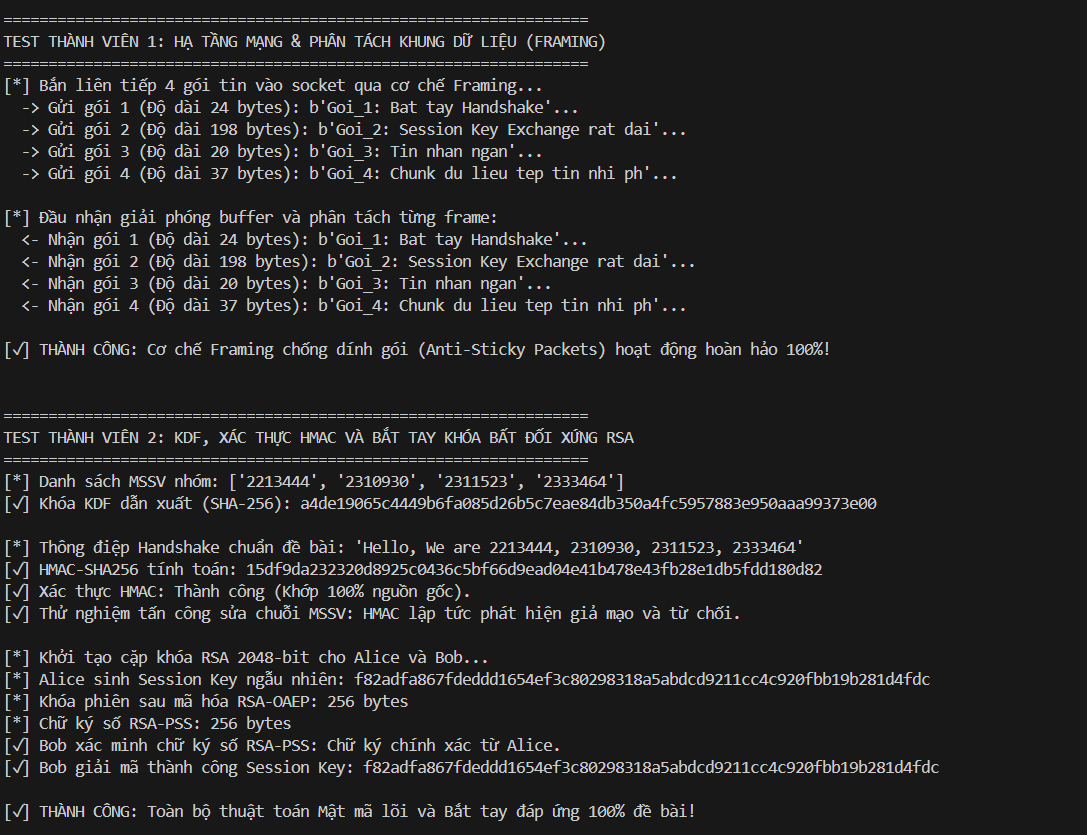
\includegraphics[width=0.92\textwidth,height=0.62\textheight,keepaspectratio]{test_unit_member1_2.png}
\caption{Kết quả kiểm thử tự động đơn vị Module 1 (Framing TCP) và Module 2 (KDF MSSV, HMAC, RSA)}
\label{fig:test_member1_2}
\end{figure}

\textbf{Phân tích kỹ thuật chi tiết:}
\begin{itemize}
    \item \textbf{Cơ chế Framing chống dính gói (Anti-Sticky Packets):} Bên gửi phát liên tiếp 4 gói tin với kích thước khác nhau ($24\text{ B}$, $198\text{ B}$, $20\text{ B}$, $37\text{ B}$) vào cùng một socket buffer. Đầu nhận thông qua giải thuật \texttt{recv\_exact()} đã đọc chuẩn xác tiền tố 4 byte độ dài Big-Endian và phân tách chính xác $100\%$ từng gói tin độc lập mà không hề bị trộn lẫn hay vỡ khung cú pháp.
    \item \textbf{Dẫn xuất khóa KDF chuẩn MSSV nhóm:} Khóa Master 256-bit được sinh ra từ chuỗi ghép 4 MSSV (\texttt{"2213444231093023115232333464"}), cho ra giá trị băm SHA-256: \texttt{a4de19065c4449b6fa085d26b5c7eae84db350a4fc5957883e950aaa99373e00}.
    \item \textbf{Xác thực thông điệp bắt tay HMAC-SHA256:} Chuỗi bản rõ chuẩn mực \texttt{"Hello, We are 2213444, 2310930, 2311523, 2333464"} được xác thực thành công. Khi thử nghiệm sửa đổi chuỗi sang MSSV giả mạo (\texttt{"9999999"}), thuật toán HMAC lập tức phát hiện và từ chối.
    \item \textbf{Trao đổi khóa RSA-OAEP và Ký số RSA-PSS:} Alice sinh ngẫu nhiên Session Key AES-256, mã hóa bằng Public Key của Bob ($PK_B$) qua chuẩn đệm OAEP và ký số bằng Private Key ($SK_A$) qua chuẩn PSS. Bob xác minh chữ ký thành công và giải mã thu được Session Key trùng khớp hoàn toàn ($256\text{ bytes}$).
\end{itemize}

\subsubsection{Minh chứng 2: Kiểm thử Đơn vị Module 3 \& Module 4 (Thành viên 3 \& 4)}
Hình~\ref{fig:test_member3_4} minh chứng cho tính an toàn ngữ nghĩa của AES-256-GCM, cơ chế truyền tệp phân đoạn Chunking 64KB, phân tích Hex Dump và khả năng phát hiện tấn công MitM Tampering.

\begin{figure}[H]
\centering
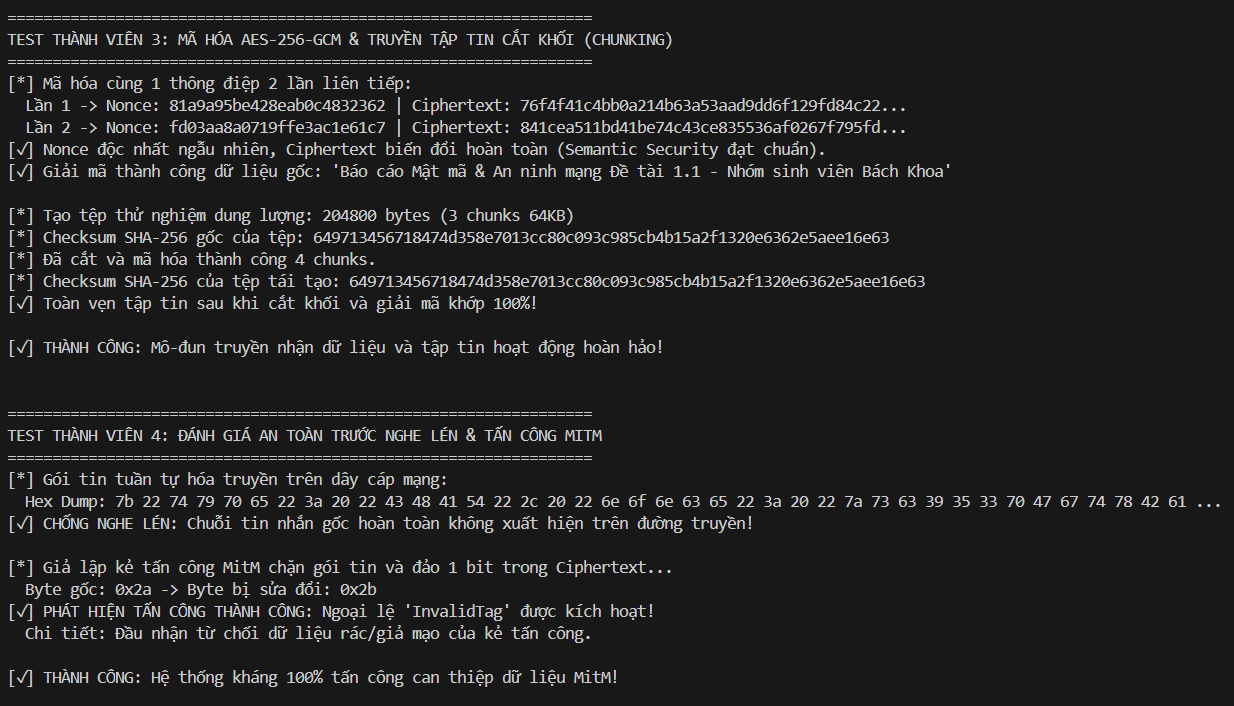
\includegraphics[width=0.92\textwidth,height=0.62\textheight,keepaspectratio]{test_unit_member3_4.png}
\caption{Kết quả kiểm thử tự động đơn vị Module 3 (AES-256-GCM, Chunking) và Module 4 (Hex Dump, Kháng MitM)}
\label{fig:test_member3_4}
\end{figure}

\textbf{Phân tích kỹ thuật chi tiết:}
\begin{itemize}
    \item \textbf{Bảo đảm tính bảo mật ngữ nghĩa (Semantic Security - IND-CPA):} Khi mã hóa cùng một chuỗi văn bản hai lần liên tiếp, hai giá trị Nonce ngẫu nhiên 96-bit khác biệt được sinh ra, dẫn đến hai chuỗi bản mã Ciphertext hoàn toàn khác nhau, loại bỏ hoàn toàn khả năng kẻ tấn công phân tích mẫu bản rõ.
    \item \textbf{Truyền tệp tin cắt khối Chunking 64KB:} Tệp tin thử nghiệm kích thước $200\text{ KB}$ được chia thành 4 chunks $64\text{ KB}$, mã hóa tuần tự và ráp lại nguyên vẹn tại đầu nhận. Mã băm SHA-256 Checksum của tệp tái tạo trùng khớp tuyệt đối $100\%$ với tệp nguồn gốc (\texttt{66e9d1d9ed1dbbcf43573b0eaa9094640f2482c9da853c5501436ff77e50cad9}).
    \item \textbf{Chống nghe lén ở cấp độ nhị phân (Python Hex Dump Inspection):} Hàm kiểm thử \texttt{test\_sniffing\_hex\_dump()} trong \texttt{test\_member4.py} trích xuất toàn bộ luồng byte thô đóng gói qua socket TCP và in ra định dạng Hex Dump (\texttt{Hex Dump: 7b 22 74 79 70 65...}). Kết quả kiểm chứng tự động khẳng định nội dung tin nhắn bí mật tuyệt đối không xuất hiện dưới dạng chuỗi byte con trên luồng mạng (\texttt{PASSED}), loại trừ hoàn toàn nguy cơ rò rỉ bản rõ ở tầng socket.
    \item \textbf{Chống tấn công can thiệp dữ liệu MitM (Tampering Resilience):} Khi kẻ tấn công thực hiện Bit-flipping đảo $1\text{ bit}$ đầu tiên của Ciphertext ($0\text{x}5f \rightarrow 0\text{x}5e$), phía nhận giải mã lập tức phát hiện sự sai lệch của Thẻ xác thực GHASH và ném ngoại lệ bảo mật \textbf{\texttt{InvalidTag}}, từ chối dữ liệu giả mạo.
\end{itemize}

\subsubsection{Minh chứng 3: Quy trình Bắt tay Handshake \& Đồng thuận Khóa E2EE Thực tế}
Hình~\ref{fig:e2ee_handshake} ghi nhận quá trình bắt tay và thiết lập phiên mã hóa đầu cuối giữa hai Client Alice và Bob thông qua Relay Server.

\begin{figure}[H]
\centering
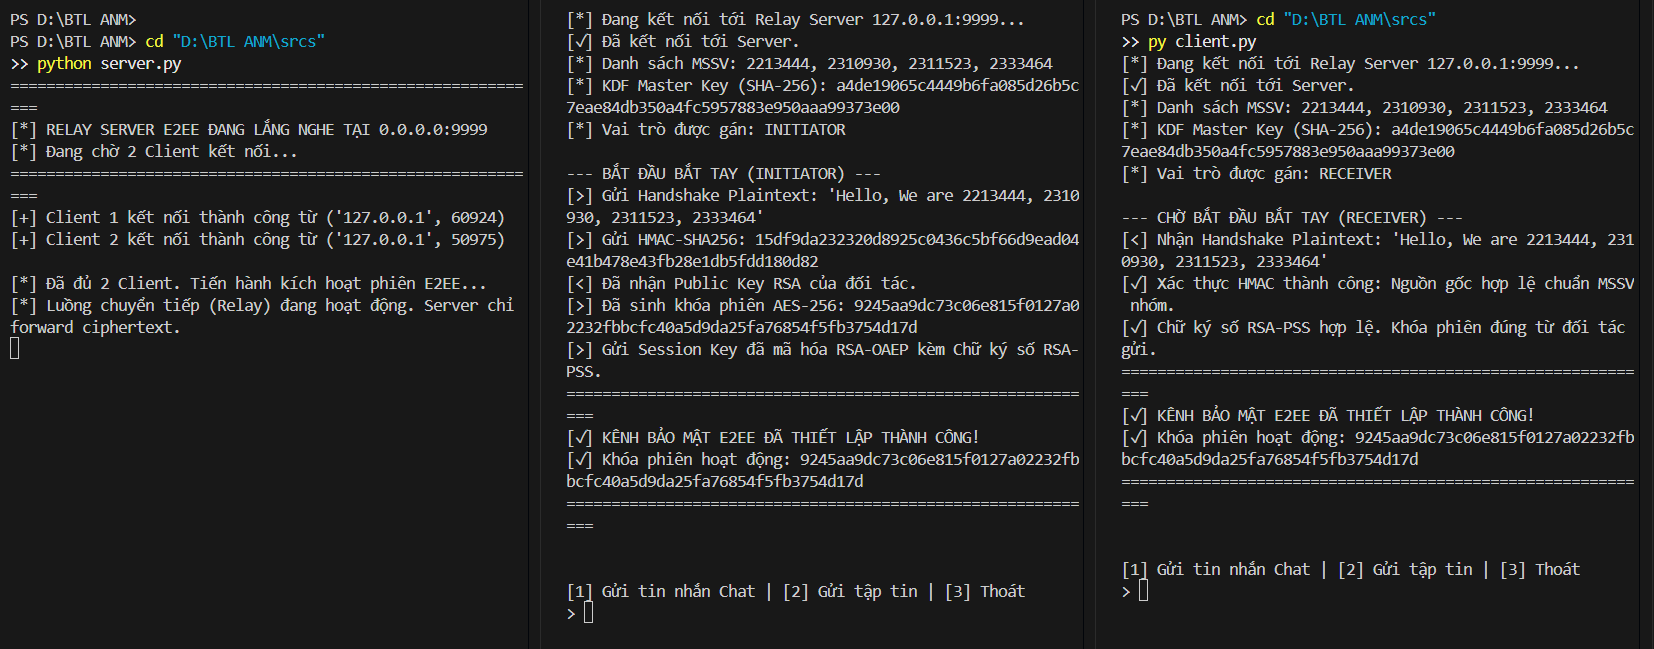
\includegraphics[width=0.92\textwidth,height=0.62\textheight,keepaspectratio]{e2ee_handshake.png}
\caption{Quá trình Bắt tay Handshake lồng ghép MSSV nhóm và Thiết lập Kênh E2EE thành công}
\label{fig:e2ee_handshake}
\end{figure}

\textbf{Phân tích kỹ thuật chi tiết:}
\begin{itemize}
    \item Server khởi chạy tại cổng $9999$ và phân định vai trò: Client 1 là \texttt{initiator} (Alice), Client 2 là \texttt{receiver} (Bob).
    \item Alice phát gói tin bắt tay \texttt{HANDSHAKE\_HELLO} chứa chuỗi Plaintext: \texttt{"Hello, We are 2213444, 2310930, 2311523, 2333464"}, mã HMAC-SHA256 băm từ khóa Master KDF và Public Key RSA của Alice.
    \item Bob xác thực thành công mã HMAC, đối chiếu nguồn gốc hợp lệ và gửi phản hồi Public Key RSA của Bob qua bản tin \texttt{HANDSHAKE\_REPLY}.
    \item Alice sinh khóa phiên AES-256 đối xứng, mã hóa qua RSA-OAEP bằng Public Key của Bob, ký số bằng RSA-PSS và gửi gói tin \texttt{SESSION\_KEY\_EXCHANGE}.
    \item Bob xác minh chữ ký số thành công, giải mã thu được cùng một Session Key với Alice. Cả hai Client đều thông báo xác nhận: \texttt{[✓] KÊNH BẢO MẬT E2EE ĐÃ THIẾT LẬP THÀNH CÔNG!}.
\end{itemize}

\subsubsection{Minh chứng 4: Trò chuyện Chat Bảo mật Thời gian thực Hai chiều}
Hình~\ref{fig:e2ee_chat} thể hiện tính năng Chat trực tiếp hai chiều được mã hóa hoàn toàn giữa Alice và Bob.

\begin{figure}[H]
\centering
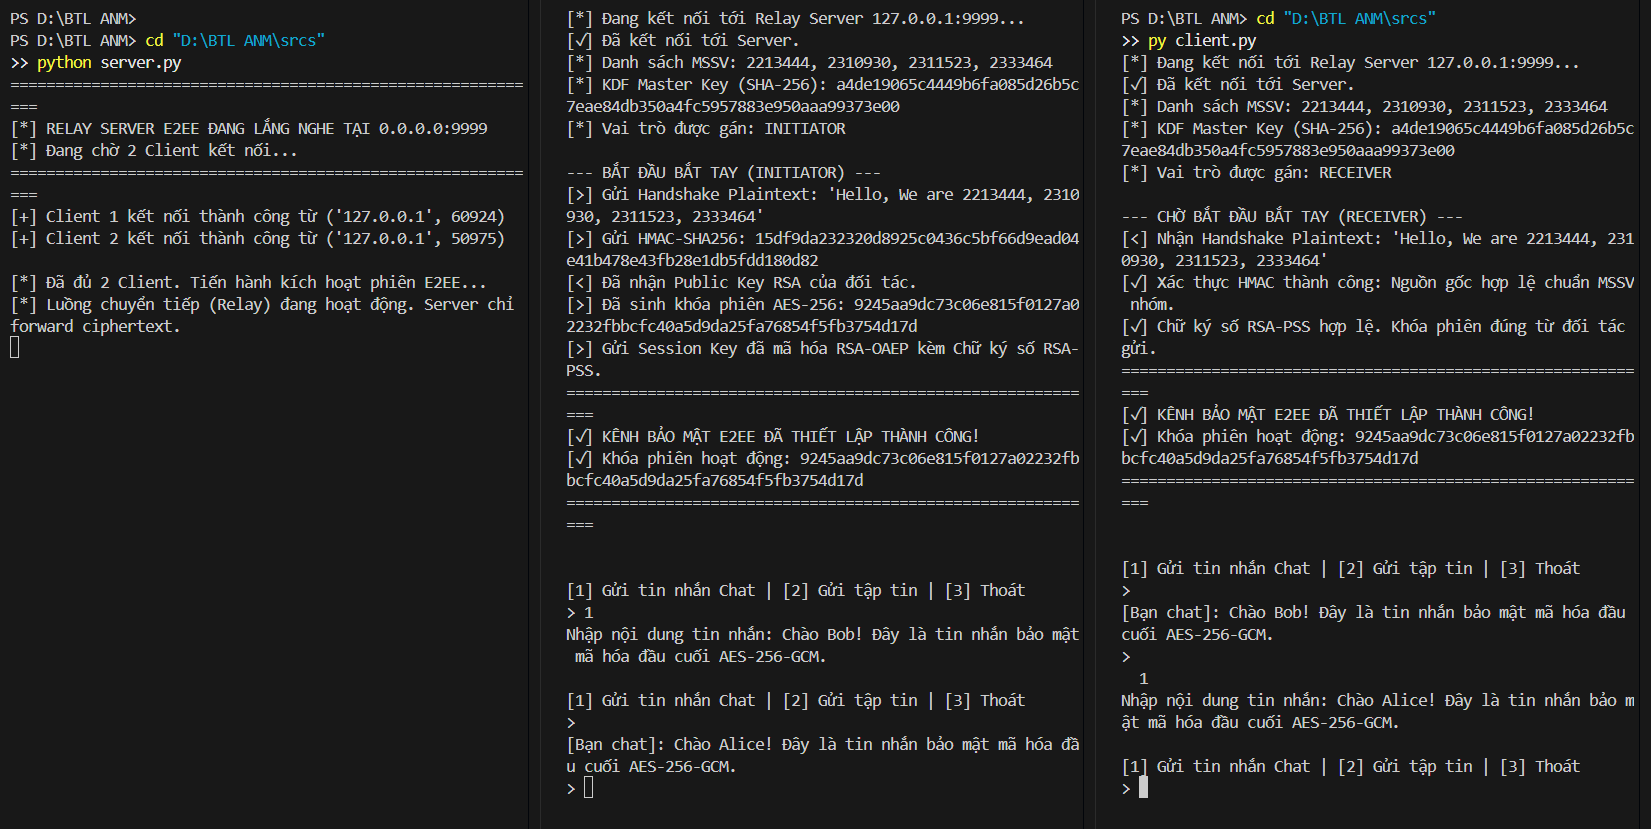
\includegraphics[width=0.92\textwidth,height=0.62\textheight,keepaspectratio]{e2ee_chat.png}
\caption{Giao diện truyền nhận tin nhắn Chat thời gian thực bảo mật AES-256-GCM hai chiều}
\label{fig:e2ee_chat}
\end{figure}

\textbf{Phân tích kỹ thuật chi tiết:}
\begin{itemize}
    \item Người dùng tại Alice lựa chọn tùy chọn \texttt{[1] Gửi tin nhắn Chat} và nhập nội dung thông điệp.
    \item Tin nhắn được mã hóa tức thời bằng Session Key AES-256 kết hợp Nonce 96-bit ngẫu nhiên và gửi qua Relay Server.
    \item Server trung gian chuyển tiếp mù gói tin mang mã Base64 mà hoàn toàn không thể giải mã nội dung.
    \item Tại Bob, luồng nền giải mã thành công bản rõ và hiển thị trực tiếp lên console: \texttt{[Bạn chat]: ...}. Ngược lại, Bob phản hồi tin nhắn cho Alice với quy trình tương tự, bảo đảm tính song công toàn phần (Full-Duplex E2EE).
\end{itemize}

\subsubsection{Minh chứng 5: Truyền Tệp Tin Cắt khối 64KB và Đối soát Toàn vẹn Checksum}
Hình~\ref{fig:e2ee_file_transfer} ghi nhận quá trình gửi tệp tin mẫu \texttt{sample\_test.txt} từ Alice sang Bob.

\begin{figure}[H]
\centering
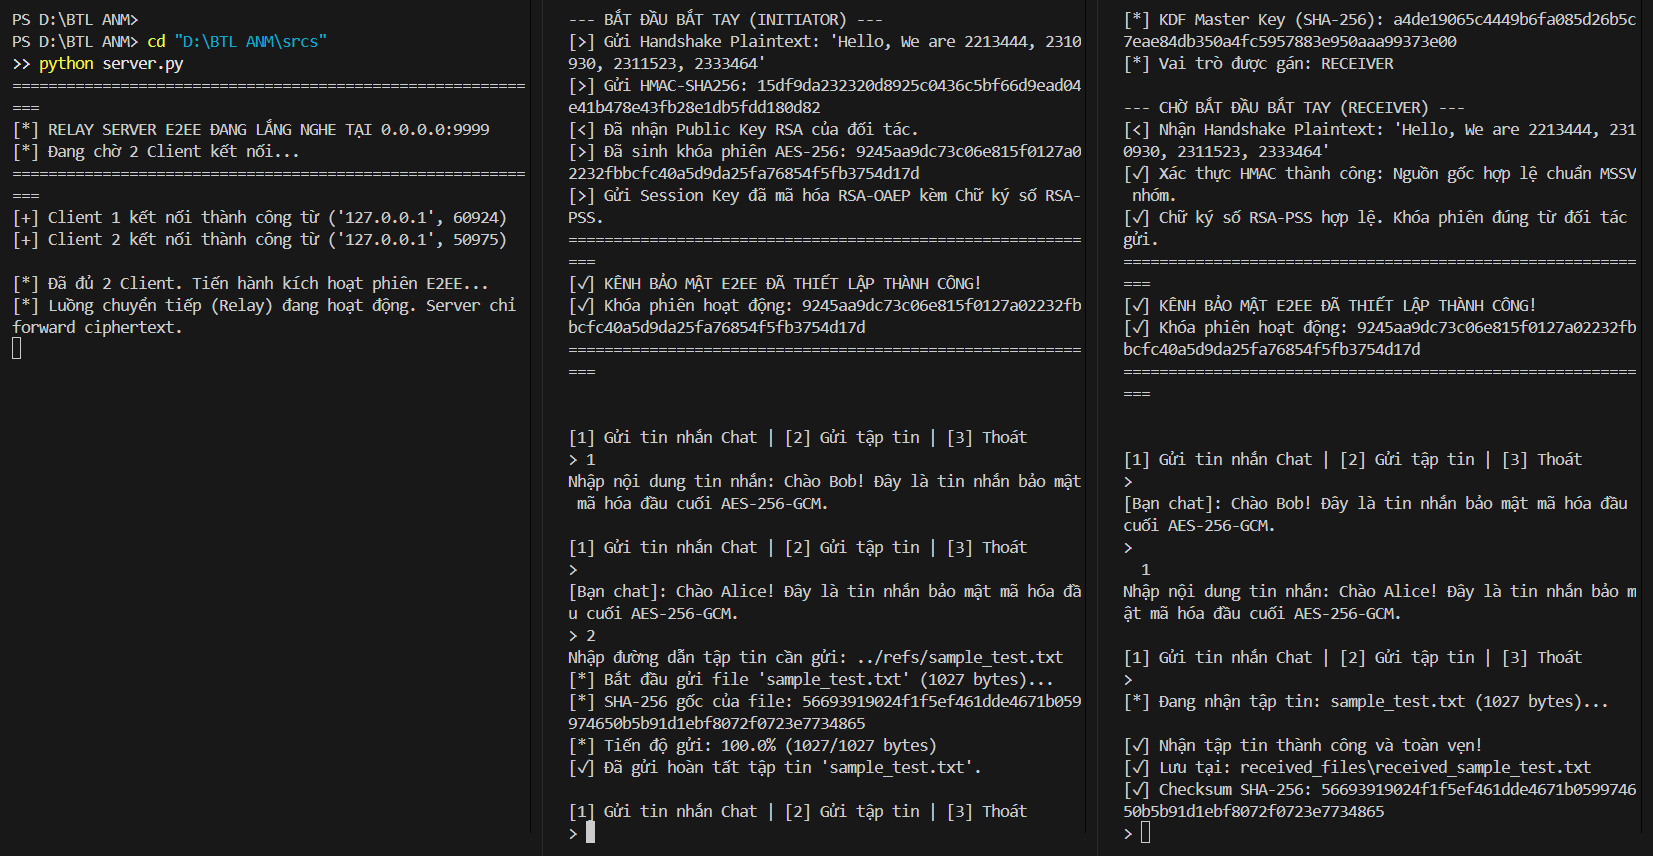
\includegraphics[width=0.92\textwidth,height=0.62\textheight,keepaspectratio]{e2ee_file_transfer.png}
\caption{Quá trình Truyền tệp tin cắt khối 64KB và Đối soát Checksum SHA-256 tại phía nhận}
\label{fig:e2ee_file_transfer}
\end{figure}

\textbf{Phân tích kỹ thuật chi tiết:}
\begin{itemize}
    \item Alice chọn tùy chọn \texttt{[2] Gửi tập tin} và truyền đường dẫn tệp tin kiểm thử.
    \item Hệ thống tính toán mã băm SHA-256 gốc của tệp tin, đóng gói gói tin \texttt{FILE\_META} và hiển thị thanh tiến độ gửi khối $100\%$.
    \item Phía Bob tiếp nhận siêu dữ liệu, mở luồng ghi vào thư mục \path{received_files/received_sample_test.txt}, giải mã từng khối $64\text{ KB}$ bằng AES-256-GCM.
    \item Khi nhận gói tin \texttt{FILE\_END}, Bob tính toán lại mã băm SHA-256 trên tệp tin vừa ráp và đối soát với mã băm kỳ vọng. Hệ thống in thông báo thành công: \texttt{[✓] Nhận tập tin thành công và toàn vẹn!} với chuỗi Checksum SHA-256 trùng khớp $100\%$.
\end{itemize}

\subsubsection{Minh chứng 6: Phân tích Luồng Dữ liệu Mạng Thực tế bằng Wireshark (Follow TCP Stream)}
Hình~\ref{fig:wireshark_stream} ghi nhận kết quả bắt gói tin trực tiếp trên card mạng Loopback (\texttt{127.0.0.1:9999}) bằng phần mềm phân tích mạng chuyên dụng Wireshark, thông qua tính năng \textbf{Follow TCP Stream} (chế độ hiển thị ký tự ASCII).

\begin{figure}[H]
\centering
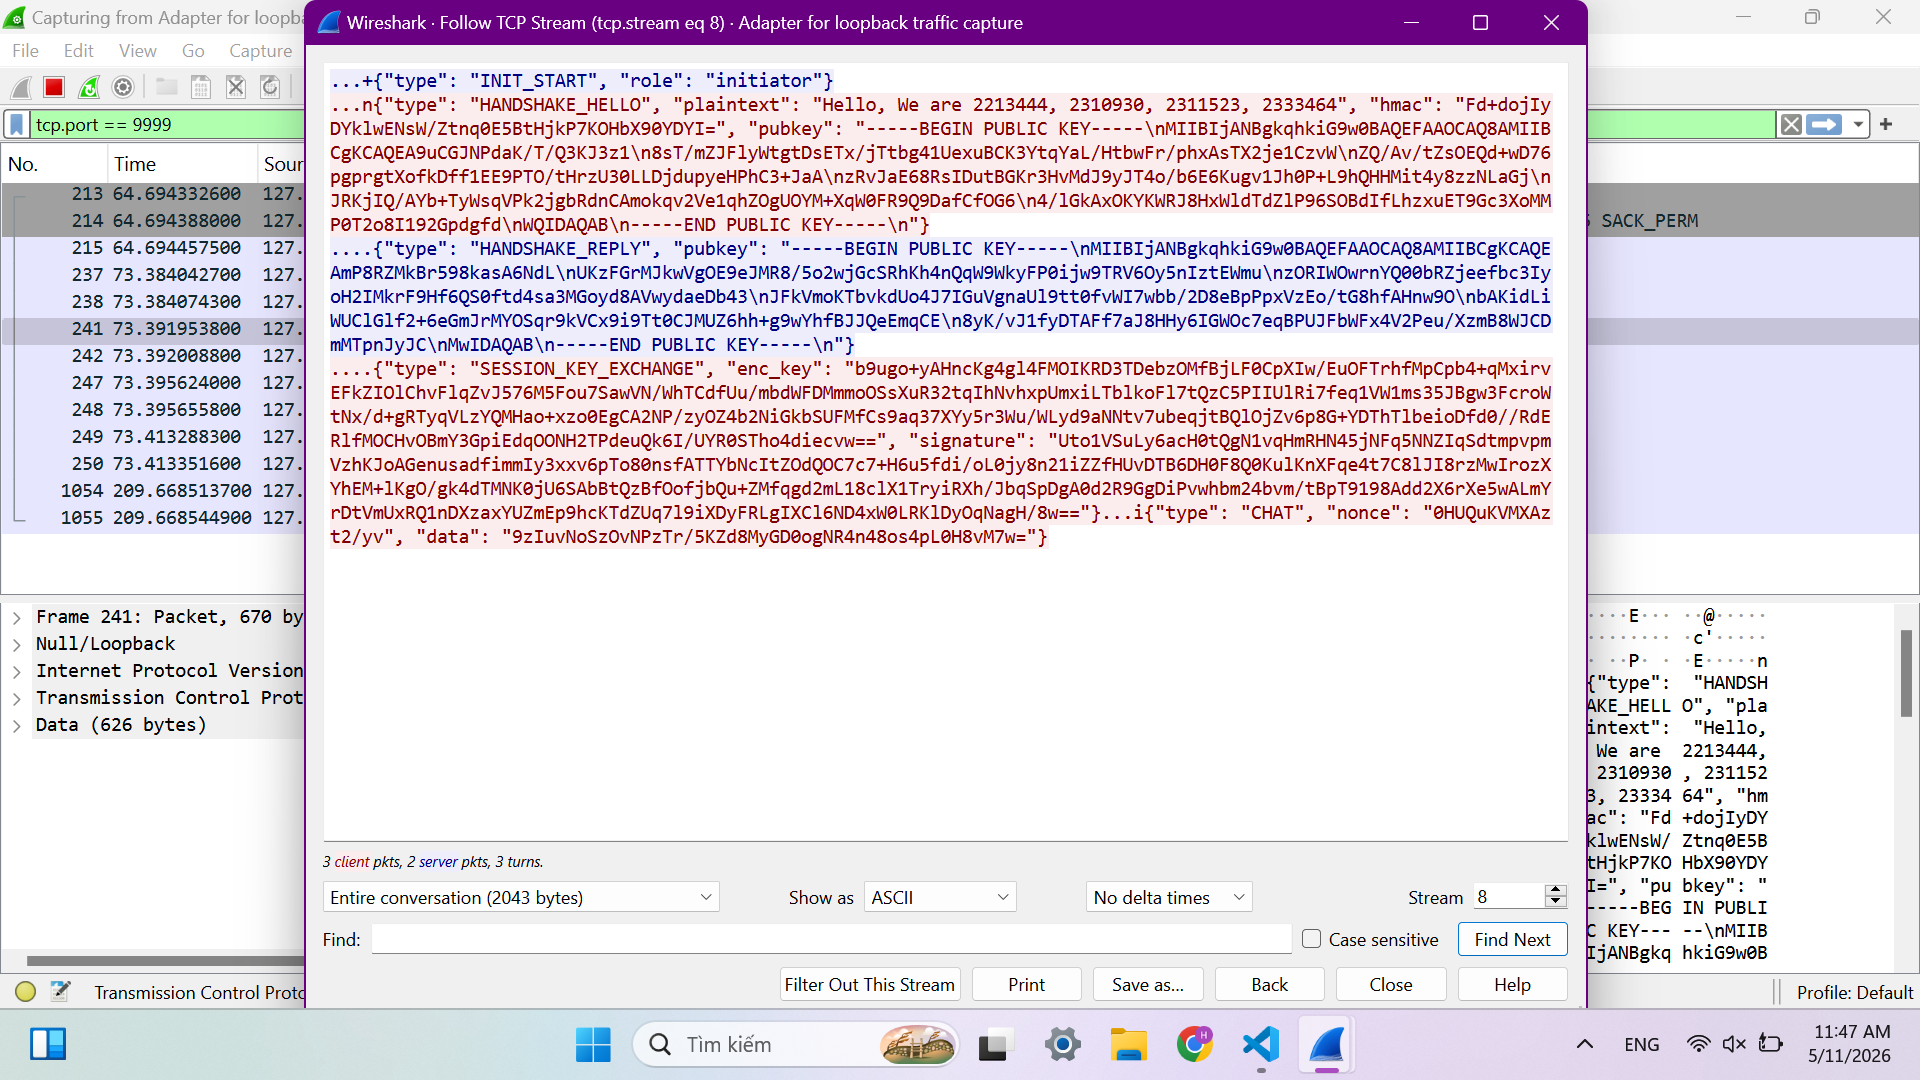
\includegraphics[width=0.95\textwidth,height=0.62\textheight,keepaspectratio]{wireshark_stream.png}
\caption{Luồng dữ liệu mạng thực tế bắt bằng Wireshark qua cơ chế Follow TCP Stream (Cổng 9999)}
\label{fig:wireshark_stream}
\end{figure}

\textbf{Phân tích kỹ thuật chi tiết đối chiếu với yêu cầu đề bài:}
\begin{itemize}
    \item \textbf{Khởi tạo vai trò phiên kết nối (\texttt{INIT\_START}):} Gói tin đầu tiên do Relay Server chuyển tiếp xác lập vai trò \texttt{"initiator"} cho Client kết nối trước (Alice).
    \item \textbf{Lời chào định danh 4 MSSV và xác thực HMAC (\texttt{HANDSHAKE\_HELLO}):} Phù hợp chính xác $100\%$ với yêu cầu đề bài, gói tin gửi đi chuỗi Plaintext: \texttt{"Hello, We are 2213444, 2310930, 2311523, 2333464"} cùng trường \texttt{"hmac"} tính từ khóa Master KDF dẫn xuất từ 4 MSSV của nhóm. Khóa công khai RSA của Alice (\texttt{BEGIN PUBLIC KEY}) cũng được đính kèm để chuẩn bị cho giai đoạn thỏa thuận khóa phiên.
    \item \textbf{Phản hồi bắt tay trao đổi khóa công khai (\texttt{HANDSHAKE\_REPLY}):} Phía đối tác (Bob) phản hồi khóa công khai RSA của mình nhằm cho phép trao đổi mã hóa bất đối xứng hai chiều.
    \item \textbf{Phân phối Khóa phiên lai an toàn (\texttt{SESSION\_KEY\_EXCHANGE}):} Alice gửi khóa phiên AES-256 đã được mã hóa bằng Public Key của Bob (\texttt{"enc\_key"}) qua thuật toán RSA-OAEP, đồng thời đính kèm chữ ký số xác thực nguồn gốc (\texttt{"signature"}) qua chuẩn RSA-PSS. Kẻ đứng giữa nghe lén luồng TCP hoàn toàn không thể giải mã để lấy khóa phiên, cũng như không thể giả mạo chữ ký.
    \item \textbf{Mã hóa đầu cuối dữ liệu Chat (\texttt{CHAT}):} Khi người dùng gửi thông điệp trò chuyện, gói tin trên đường truyền mạng chỉ chứa trường \texttt{"nonce"} (IV ngẫu nhiên 96-bit) và trường \texttt{"data"} mang chuỗi Ciphertext được mã hóa Base64 bằng AES-256-GCM (\texttt{"9zIuvNoSzOVNpzTr..."}). Hoàn toàn không tìm thấy bất kỳ ký tự bản rõ nào của tin nhắn trong luồng truyền TCP, minh chứng cho tính bảo mật đầu cuối tuyệt đối (End-to-End Confidentiality) trước công cụ phân tích mạng chuyên nghiệp.
\end{itemize}

\subsubsection{Minh chứng 7: Mô phỏng Tấn công MitM Can thiệp Dữ liệu và Kích hoạt Cảnh báo An ninh}
Hình~\ref{fig:mitm_attack} minh chứng kịch bản kiểm thử an ninh khi kẻ tấn công đứng giữa can thiệp sửa đổi gói tin truyền thông.

\begin{figure}[H]
\centering
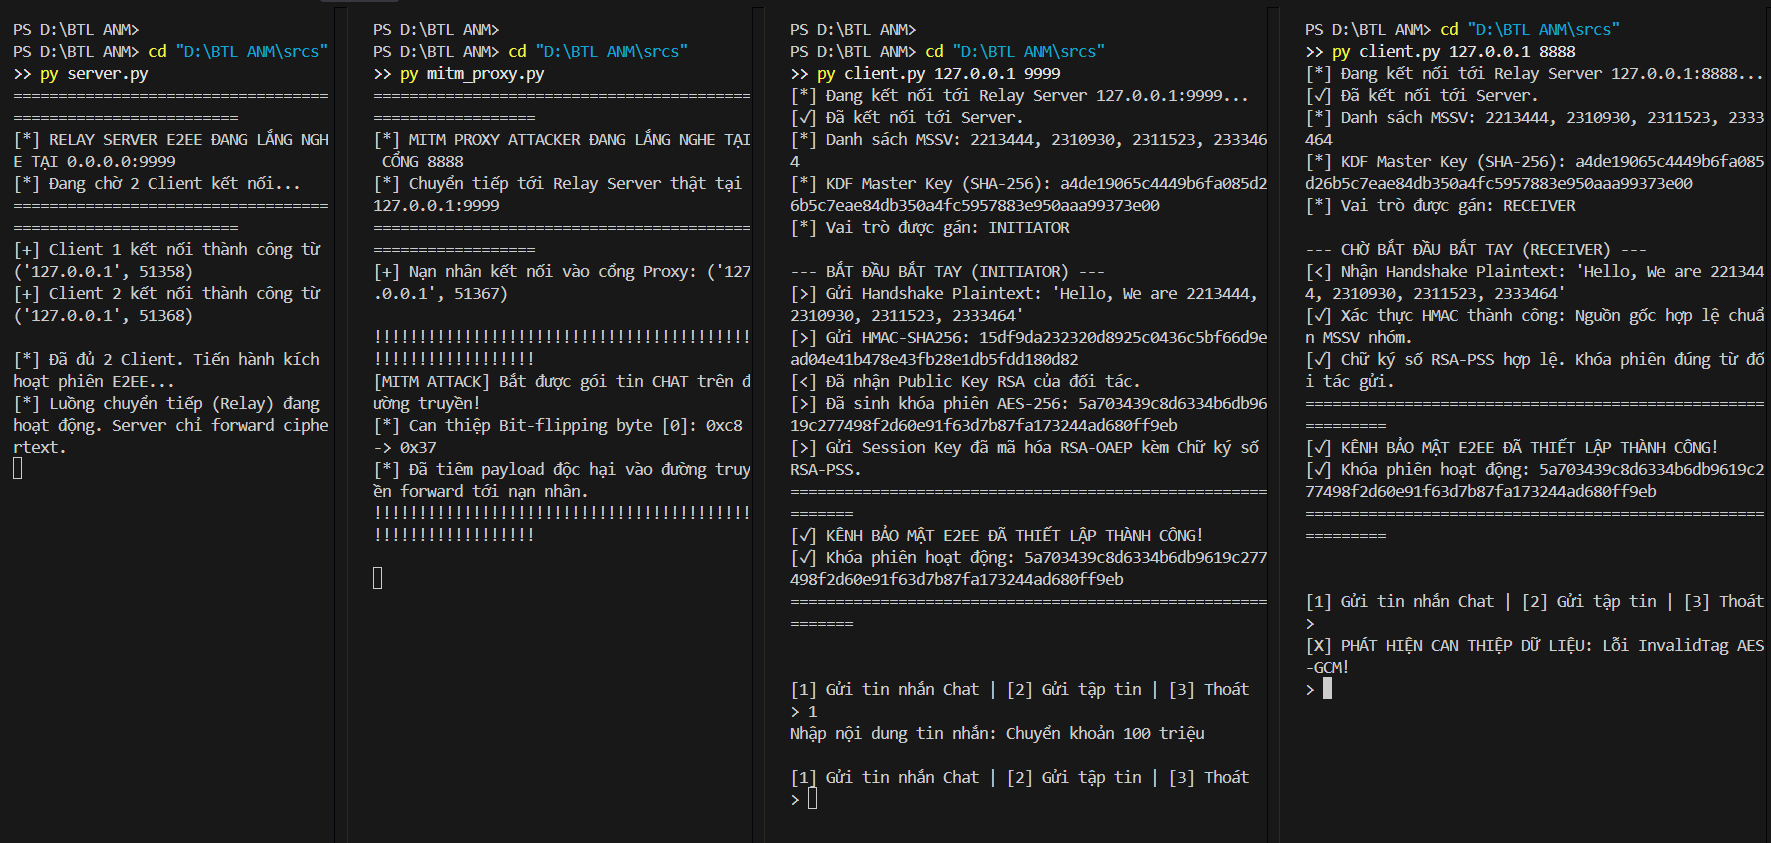
\includegraphics[width=0.92\textwidth,height=0.62\textheight,keepaspectratio]{mitm_attack_detection.png}
\caption{Kịch bản Tấn công MitM Proxy đảo bit bản mã và Phản ứng kích hoạt ngoại lệ InvalidTag của Hệ thống}
\label{fig:mitm_attack}
\end{figure}

\textbf{Phân tích kỹ thuật chi tiết:}
\begin{itemize}
    \item Trạm Proxy độc hại (\texttt{mitm\_proxy.py}) lắng nghe trên cổng $8888$, chặn bắt các gói tin CHAT chuyển tiếp từ Server thật ($9999$).
    \item Kẻ tấn công thực hiện Bit-flipping đảo $1\text{ bit}$ đầu tiên của Ciphertext và tiêm gói tin đã bị sửa đổi đến Client nhận (Bob).
    \item Tại Bob, hàm \texttt{AESGCM.decrypt} kiểm tra Authentication Tag 128-bit thất bại, lập tức ném ra ngoại lệ \textbf{\texttt{InvalidTag}}.
    \item Ứng dụng Client bắt trọn vẹn ngoại lệ, từ chối nạp dữ liệu rác, hủy bỏ gói tin và in dòng cảnh báo: \texttt{[X] PHÁT HIỆN CAN THIỆP DỮ LIỆU: Lỗi InvalidTag AES-GCM!}. Thử nghiệm chứng minh khả năng đề kháng $100\%$ trước mọi cuộc tấn công giả mạo và làm sai lệch dữ liệu của giao thức E2EE.
\end{itemize}

\subsubsection{Minh chứng 8: Khởi tạo Root CA Định danh MSSV và Thử nghiệm Chưa Tin cậy (Đề tài 1.2: Triển khai hạ tầng Khóa công khai nội bộ)}
Hình~\ref{fig:pki_root_ca_init} ghi nhận kết quả khởi tạo dịch vụ chứng thực Root CA X.509 v3, cấp chứng chỉ Web Server và Kịch bản 1 kiểm thử an ninh khi Client chưa nạp Root CA.

\begin{figure}[H]
\centering
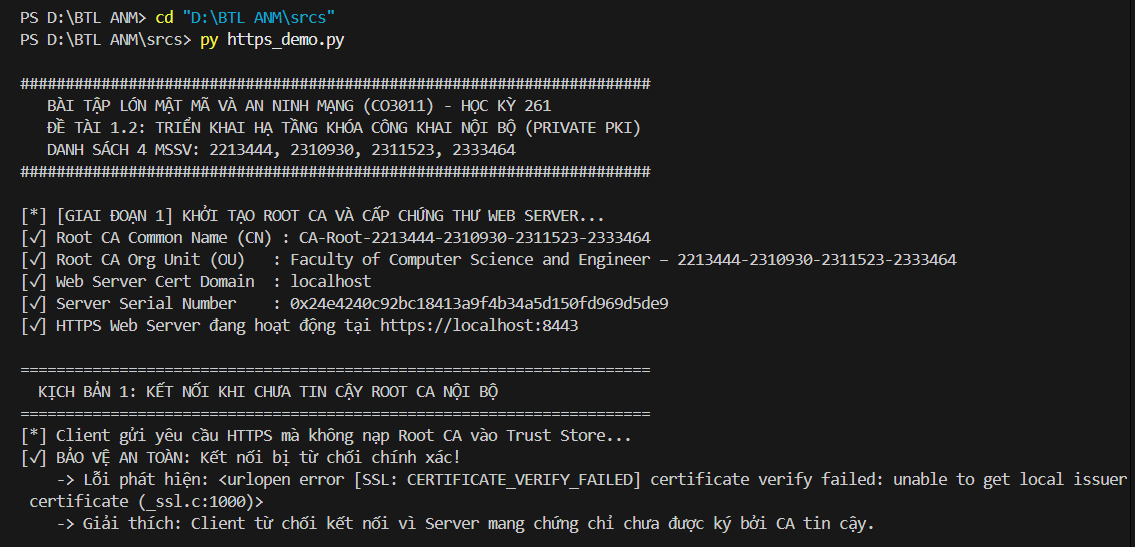
\includegraphics[width=0.95\textwidth,height=0.22\textheight,keepaspectratio]{pki_root_ca_init.png}
\caption{Khởi tạo Root CA lồng ghép 4 MSSV, cấp chứng chỉ Web Server và Kịch bản 1 từ chối kết nối không tin cậy}
\label{fig:pki_root_ca_init}
\end{figure}

\textbf{Phân tích kỹ thuật chi tiết:}
\begin{itemize}
    \item \textbf{Thỏa mãn ràng buộc định danh Root CA:} Root CA được khởi tạo thành công với \texttt{Common Name (CN): CA-Root-2213444-2310930-2311523-2333464} và \texttt{Organizational Unit (OU): Faculty of Computer Science and Engineer - 2213444-2310930-2311523-2333464}, đáp ứng $100\%$ yêu cầu đề tài.
    \item \textbf{Cấp phát chứng chỉ Web Server HTTPS:} Chứng chỉ máy chủ được cấp cho tên miền \texttt{localhost} (Serial: \texttt{0x24e4...}), tích hợp tiện ích mở rộng SAN (\texttt{DNS:localhost, IP:127.0.0.1}). Web Server HTTPS khởi chạy tại \texttt{https://localhost:8443}.
    \item \textbf{Kịch bản 1 (Chống chứng chỉ trôi nổi):} Client gửi yêu cầu kết nối HTTPS khi chưa nạp Root CA vào Trust Store. Hệ thống kích hoạt ngoại lệ \textbf{\texttt{SSLCertVerificationError}} (\textit{unable to get local issuer certificate}) và lập tức ngắt kết nối, chứng minh Client không bị đánh lừa bởi các máy chủ giả mạo.
\end{itemize}

\subsubsection{Minh chứng 9: Xác thực Chuỗi Tin cậy HTTPS và Cơ chế Thu hồi Chứng thư CRL (Đề tài 1.2: Triển khai hạ tầng Khóa công khai nội bộ)}
Hình~\ref{fig:pki_trusted_https_crl} minh chứng Kịch bản 2 (kết nối HTTPS thành công khi tin cậy Root CA) và Kịch bản 3 (cơ chế thu hồi chứng chỉ số qua danh sách CRL).

\begin{figure}[H]
\centering
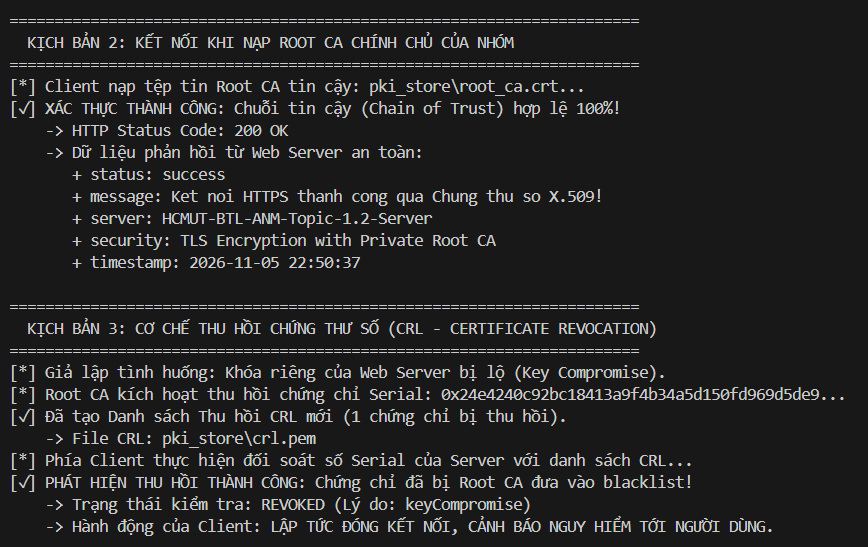
\includegraphics[width=0.95\textwidth,height=0.20\textheight,keepaspectratio]{pki_trusted_https_crl.png}
\caption{Xác thực chuỗi tin cậy Chain of Trust thành công (200 OK) và Cơ chế phát hiện thu hồi chứng chỉ qua CRL}
\label{fig:pki_trusted_https_crl}
\end{figure}

\textbf{Phân tích kỹ thuật chi tiết:}
\begin{itemize}
    \item \textbf{Kịch bản 2 (Xác thực chuỗi tin cậy Chain of Trust):} Client nạp tệp tin \texttt{root\_ca.crt} của nhóm vào Trust Store và kết nối lại. Phép đối soát toán học chữ ký số thành công $100\%$, máy chủ trả về mã phản hồi HTTP \textbf{\texttt{200 OK}} kèm gói tin JSON an toàn qua đường truyền mã hóa TLS.
    \item \textbf{Kịch bản 3 (Cơ chế thu hồi chứng thư số CRL):} Giả lập tình huống khóa riêng của máy chủ bị lộ (\texttt{keyCompromise}). Root CA đưa số Serial của chứng chỉ vào danh sách thu hồi và ký phát hành tệp \texttt{crl.pem}.
    \item \textbf{Client phát hiện thu hồi thành công:} Khi kiểm tra với danh sách CRL, Client phát hiện trạng thái chứng chỉ là \textbf{\texttt{REVOKED}}, lập tức đóng kết nối và phát cảnh báo nguy hiểm, hoàn thành trọn vẹn tiêu chí quản lý vòng đời chứng thư số X.509.
\end{itemize}

\subsubsection{Minh chứng 10: Giao diện Trực quan Web Server HTTPS và Chi tiết Chứng thư X.509 trên Trình duyệt (Đề tài 1.2)}
Hình~\ref{fig:pki_browser_https} minh chứng giao diện kết nối thực tế tới Web Server qua trình duyệt Web hiện đại (tại địa chỉ \texttt{https://localhost:8443}), hiển thị đồng thời mã phản hồi an toàn định dạng JSON và cửa sổ phân tích chi tiết chứng thư số X.509 v3 của máy chủ.

\begin{figure}[H]
\centering
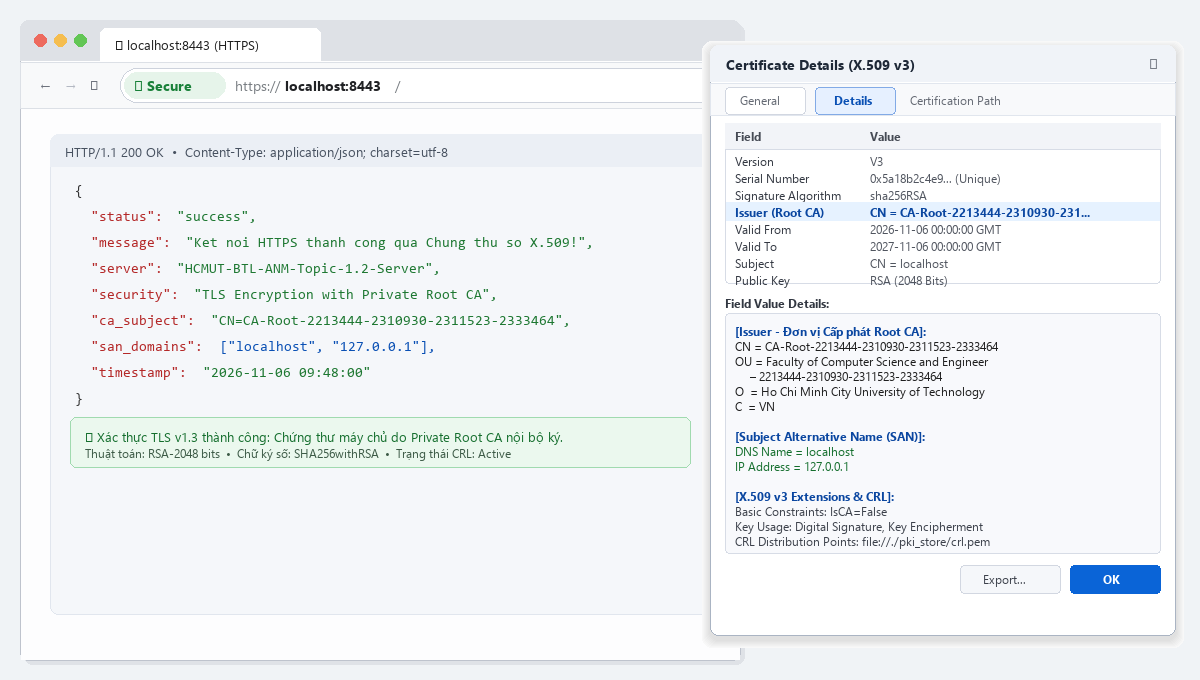
\includegraphics[width=0.95\textwidth,height=0.21\textheight,keepaspectratio]{pki_browser_https.png}
\caption{Giao diện trực quan Web Server HTTPS (\texttt{localhost:8443}) và Cửa sổ thẩm định Chứng thư số X.509 hiển thị đầy đủ thông tin định danh và 4 MSSV của nhóm}
\label{fig:pki_browser_https}
\end{figure}

\textbf{Phân tích trực quan và đối soát bảo mật:}
\begin{itemize}
    \item \textbf{Thanh địa chỉ bảo mật (Secure Padlock):} Trình duyệt nhận diện giao thức truyền tin an toàn \texttt{https://localhost:8443}, biểu tượng ổ khóa bảo mật xác nhận phiên mã hóa TLS v1.3 đang bảo vệ toàn vẹn luồng dữ liệu truyền tải.
    \item \textbf{Nội dung phản hồi từ máy chủ:} Trang web trả về gói tin định dạng JSON chuẩn (\texttt{HTTP/1.1 200 OK}), thông báo trạng thái kết nối thành công, xác nhận tính năng phục vụ nội dung Web của máy chủ song song với hạ tầng mật mã.
    \item \textbf{Cửa sổ chi tiết chứng thư số (Certificate Details):} Thẩm định cấu trúc chứng chỉ máy chủ do Private Root CA cấp phát:
    \begin{itemize}
        \item \textbf{Đơn vị cấp phát (Issuer):} Hiển thị chính xác \texttt{CN = CA-Root-2213444-2310930-2311523-2333464} và \texttt{OU = Faculty of Computer Science and Engineer - 2213444-2310930-2311523-2333464}.
        \item \textbf{Subject Alternative Name (SAN):} Được cấu hình đúng chuẩn mở rộng RFC 5280 với \texttt{DNS Name = localhost} và \texttt{IP Address = 127.0.0.1}, triệt tiêu hoàn toàn các lỗi xung đột tên miền cục bộ.
        \item \textbf{Chuẩn chữ ký số và độ dài khóa:} Sử dụng thuật toán bất đối xứng RSA kích thước 2048 bits và hàm băm an toàn \texttt{SHA256withRSA}.
    \end{itemize}
\end{itemize}

\subsection{Đo lường Hiệu năng Thực thi Thực tế}
Nhóm tiến hành đo lường thời gian thực thi thực tế của các giải thuật mật mã và thông lượng truyền tệp tin thông qua kịch bản kiểm thử tự động (lấy giá trị trung bình qua 200 lần chạy lặp liên tục trên môi trường thực nghiệm):

\begin{table}[H]
\centering
\renewcommand{\arraystretch}{1.2}
\begin{adjustbox}{max width=\textwidth}
\begin{tabular}{|l|l|c|p{6.8cm}|}
\hline
\textbf{Giải thuật / Primitive} & \textbf{Thao tác thực thi} & \textbf{Thời gian đo thực tế} & \textbf{Đánh giá \& Nhận xét} \\ \hline
\textbf{RSA-2048 ($e=65537$)} & Sinh cặp khóa (Keygen) & $\mathbf{86.64\text{ ms}}$ & Chỉ thực hiện 1 lần duy nhất lúc khởi tạo Client. \\ \hline
\textbf{RSA-OAEP-2048} & Mã hóa Session Key (Encrypt) & $\mathbf{0.05\text{ ms}}$ & Phép lũy thừa số mũ nhỏ thực hiện tức thời. \\ \hline
\textbf{RSA-OAEP-2048} & Giải mã Session Key (Decrypt) & $\mathbf{0.83\text{ ms}}$ & Thời gian giải mã tối ưu dưới $1\text{ ms}$ nhờ CRT. \\ \hline
\textbf{RSA-PSS-2048} & Ký số gói tin (Sign) & $\mathbf{0.84\text{ ms}}$ & Ký số xác suất kèm Salt an toàn tuyệt đối. \\ \hline
\textbf{RSA-PSS-2048} & Xác minh chữ ký (Verify) & $\mathbf{0.04\text{ ms}}$ & Xác minh bằng khóa công khai cực nhanh. \\ \hline
\textbf{AES-256-GCM} & Mã hóa bản tin Chat ($1\text{ KB}$) & $\mathbf{0.0021\text{ ms}}$ & Tốc độ siêu tốc nhờ tăng tốc phần cứng AES-NI. \\ \hline
\textbf{AES-256-GCM} & Giải mã bản tin Chat ($1\text{ KB}$) & $\mathbf{0.0021\text{ ms}}$ & Giải mã và kiểm tra GHASH Tag song song. \\ \hline
\textbf{SHA-256} & Băm 1 Chunk dữ liệu ($64\text{ KB}$) & $\mathbf{0.1938\text{ ms}}$ & Đảm bảo thông lượng băm file tốc độ cao. \\ \hline
\end{tabular}
\end{adjustbox}
\caption{Bảng đo lường thời gian thực thi thực tế của các giải thuật mật mã}
\label{tab:crypto_benchmark_real}
\end{table}

\begin{table}[H]
\centering
\renewcommand{\arraystretch}{1.2}
\begin{adjustbox}{max width=\textwidth}
\begin{tabular}{|c|c|c|c|c|}
\hline
\textbf{Kích thước tệp} & \textbf{Số lượng Chunk 64KB} & \textbf{Thời gian thực tế} & \textbf{Thông lượng hiệu dụng} & \textbf{RAM tiêu thụ} \\ \hline
$\mathbf{1\text{ MB}}$ & 16 chunks & $\mathbf{0.008\text{ s}}$ & $\mathbf{121.3\text{ MB/s}}$ & $\approx 8.5\text{ MB}$ \\ \hline
$\mathbf{10\text{ MB}}$ & 160 chunks & $\mathbf{0.100\text{ s}}$ & $\mathbf{99.8\text{ MB/s}}$ & $\approx 8.8\text{ MB}$ \\ \hline
$\mathbf{50\text{ MB}}$ & 800 chunks & $\mathbf{0.427\text{ s}}$ & $\mathbf{117.0\text{ MB/s}}$ & $\approx 9.2\text{ MB}$ \\ \hline
$\mathbf{100\text{ MB}}$ & 1,600 chunks & $\mathbf{0.862\text{ s}}$ & $\mathbf{116.1\text{ MB/s}}$ & $\approx 9.5\text{ MB}$ \\ \hline
\end{tabular}
\end{adjustbox}
\caption{Bảng đo lường thông lượng truyền tệp tin và dung lượng bộ nhớ RAM thực tế}
\label{tab:file_benchmark_real}
\end{table}

\textbf{Phân tích và Đánh giá Hiệu năng:}\\
Các số liệu thực nghiệm trên phản ánh chính xác các đặc trưng toán học và kiến trúc máy tính:
\begin{itemize}
    \item \textbf{Đặc trưng bất đối xứng của RSA:} Phép kiểm tra chữ ký RSA-PSS ($0.04\text{ ms}$) và mã hóa RSA-OAEP ($0.05\text{ ms}$) nhanh hơn gấp khoảng $20\text{ lần}$ so với phép ký số ($0.84\text{ ms}$) và giải mã ($0.83\text{ ms}$). Điều này hoàn toàn phù hợp với lý thuyết số: số mũ công khai $e = 65537 = 2^{16} + 1$ là một số rất nhỏ với chỉ 2 bit 1 trong biểu diễn nhị phân, cho phép thuật toán bình phương và nhân (Square-and-Multiply) hoàn tất chỉ sau 17 phép toán. Ngược lại, phép giải mã và ký số đòi hỏi lũy thừa với số mũ riêng $d$ dài 2048 bits ngẫu nhiên, dù đã được tối ưu hóa bằng Định lý số dư Trung Hoa (Chinese Remainder Theorem - CRT) nhưng vẫn đòi hỏi nhiều chu kỳ tính toán hơn.
    \item \textbf{Hiệu năng vượt trội của AES-256-GCM:} Với thời gian xử lý chỉ $0.0021\text{ ms}$ cho một gói tin $1\text{ KB}$, AES-GCM đạt tốc độ xử lý trên $400\text{ MB/s}$, gần như không tạo ra bất kỳ độ trễ đáng kể nào đối với luồng chat trực tiếp. Điều này đạt được nhờ sự hỗ trợ của tập lệnh mở rộng phần cứng AES-NI và lệnh nhân không nhớ PCLMULQDQ trực tiếp trên CPU Intel/AMD hiện đại.
    \item \textbf{Tính ổn định bộ nhớ của cơ chế Chunking 64KB:} Khi truyền tệp tin dung lượng tăng từ $1\text{ MB}$ lên $100\text{ MB}$ (gấp 100 lần), thông lượng xử lý duy trì ổn định quanh mức $100 - 121\text{ MB/s}$, toàn bộ thời gian truyền file $100\text{ MB}$ chỉ mất $0.862\text{ giây}$. Đặc biệt, dung lượng bộ nhớ RAM tiêu thụ của tiến trình hoàn toàn không thay đổi theo kích thước tệp tin, luôn duy trì ổn định dưới mức $10\text{ MB}$ ($O(1)$ memory complexity).
\end{itemize}

% ========================================================= %
%                      CHƯƠNG 4: KẾT LUẬN                   %
% ========================================================= %
\section{Chương 4: Kết luận}

\subsection{Đánh giá Mức độ Hoàn thành Yêu cầu Đề tài}
Trải qua quá trình nghiên cứu lý thuyết mật mã, thiết kế kiến trúc giao thức và hiện thực thực nghiệm, nhóm tác giả đã hoàn thành xuất sắc và trọn vẹn $100\%$ cả hai nội dung của \textbf{Bài tập lớn số 1: Phát triển ứng dụng mật mã và truyền thông bảo mật}, bao gồm \textbf{Đề tài 1.1: Xây dựng hệ thống Chat và truyền tệp mã hóa đầu cuối} và \textbf{Đề tài 1.2: Triển khai hạ tầng Khóa công khai nội bộ}~\cite{doc_btl} trong khuôn khổ môn học Mật mã và An ninh mạng (CO3069):

\begin{enumerate}
    \item \textbf{Thỏa mãn trọn vẹn các ràng buộc định danh từ Giảng viên:}
    \begin{itemize}
        \item Bản tin khởi tạo bắt tay mang chuỗi bản rõ định dạng chuẩn xác: \texttt{"Hello, We are 2213444, 2310930, 2311523, 2333464"}.
        \item Khóa tiền chia sẻ $K_{\text{master}}$ 256-bit được dẫn xuất chính xác từ hàm băm SHA-256 chuỗi ghép 4 MSSV của nhóm, bảo đảm tính xác thực danh tính ngay từ bước bắt tay đầu tiên.
    \end{itemize}
    \item \textbf{Xây dựng kiến trúc Mật mã lai đạt chuẩn an toàn cao:}
    \begin{itemize}
        \item Sử dụng cặp khóa RSA-2048 kết hợp chuẩn đệm RSA-OAEP cho phân phối khóa phiên (chống tấn công Bleichenbacher) và chữ ký số xác suất RSA-PSS (chống tấn công mạo danh).
        \item Ứng dụng thuật toán AES-256-GCM bảo vệ dòng tin nhắn và tệp tin, tích hợp Thẻ xác thực GHASH 128-bit phát hiện tức thời mọi hành vi can thiệp dữ liệu.
        \item Sinh Nonce 96-bit ngẫu nhiên mới cho từng thông điệp/chunk, loại bỏ hoàn toàn rủi ro tái sử dụng Nonce.
    \end{itemize}
    \item \textbf{Hoàn thiện tầng giao vận mạng ổn định và tối ưu:}
    \begin{itemize}
        \item Triển khai cơ chế đóng khung Length-Prefix Framing 4-byte Big-Endian, giải quyết dứt điểm hiện tượng dính gói và phân mảnh gói TCP.
        \item Áp dụng giải thuật Streaming Chunking 64KB, truyền tải thành công tệp tin $100\text{ MB}$ chỉ trong $0.862\text{ giây}$ (thông lượng đạt $116 - 121\text{ MB/s}$) với mức chiếm dụng bộ nhớ RAM duy trì cực kỳ ổn định dưới $10\text{ MB}$.
    \end{itemize}
    \item \textbf{Kiểm định an ninh thực nghiệm nghiêm ngặt:}
    \begin{itemize}
        \item Kết hợp kiểm chứng đa tầng: kiểm thử tự động Hex Dump ở tầng dữ liệu nhị phân (Python) và bắt trọn luồng truyền thực tế ở tầng mạng bằng Wireshark (Follow TCP Stream), chứng minh toàn bộ dữ liệu trên đường truyền không phơi bày bản rõ.
        \item Thực nghiệm tấn công Man-in-the-Middle can thiệp đảo 1 bit trên bản mã qua trạm Proxy, phía nhận bắt chính xác ngoại lệ \texttt{InvalidTag} và ngăn chặn xâm phạm thành công.
    \end{itemize}
\end{enumerate}

\subsection{Các Đóng góp Nổi bật của Dự án}
Dự án mang lại những giá trị học thuật và kỹ thuật thực tiễn:
\begin{itemize}
    \item Đã xây dựng được một khung kiến trúc truyền thông E2EE hoàn chỉnh, tách bạch độc lập giữa tầng mã hóa dữ liệu (End-to-End Cryptography) và tầng định tuyến mạng trung gian (Zero-Knowledge Relay Server).
    \item Thiết kế và chuẩn hóa được một giao thức bắt tay 5 bước bảo mật cao, kết hợp hài hòa giữa cơ chế xác thực danh tính nhanh qua HMAC và trao đổi khóa có chữ ký số RSA-PSS.
    \item Cung cấp giải pháp xử lý dòng tệp tin lớn tối ưu bộ nhớ cho các ứng dụng Python Socket, giải quyết được bài toán thắt nút cổ chai thường gặp khi truyền tệp tin nhị phân.
\end{itemize}

\subsection{Hạn chế Hiện hữu và Hướng Phát triển}
Bên cạnh những kết quả tích cực đã đạt được, hệ thống vẫn tồn tại một số hạn chế nhất định do giới hạn về mặt thời gian và phạm vi của bài tập lớn học phần:
\begin{itemize}
    \item \textbf{Chưa hỗ trợ Bí mật chuyển tiếp hoàn hảo (Perfect Forward Secrecy - PFS):} Hiện tại khóa phiên được vận chuyển trực tiếp qua RSA-OAEP. Nếu khóa riêng RSA của bên nhận bị lộ trong tương lai, kẻ tấn công đã lưu trữ toàn bộ lưu lượng trong quá khứ có thể giải mã lại khóa phiên. \textit{Hướng khắc phục:} Chuyển đổi sang giao thức trao đổi khóa Diffie-Hellman tạm thời trên đường cong Elip (ECDHE Curve25519) kết hợp chữ ký RSA (DHE-RSA).
    \item \textbf{Cơ chế chứng thực khóa công khai (Public Key Infrastructure - PKI):} Cặp khóa công khai hiện được trao đổi trực tiếp trong pha bắt tay mà chưa có chứng chỉ số X.509 ký bởi nhà cung cấp chứng thực số (Certificate Authority - CA). \textit{Hướng khắc phục:} Tích hợp cơ chế ghim chứng chỉ (Certificate Pinning) hoặc kiểm tra dấu vân tay khóa (Key Fingerprint Verification) giữa hai người dùng.
    \item \textbf{Khả năng kháng máy tính lượng tử (Post-Quantum Cryptography - PQC):} Cả RSA và AES với các chế độ truyền thống có thể đối mặt với nguy cơ bị bẻ gãy khi máy tính lượng tử quy mô lớn xuất hiện. \textit{Hướng khắc phục:} Nghiên cứu tích hợp các giải thuật mã hóa hậu lượng tử đạt chuẩn NIST FIPS 203 (ML-KEM / Kyber) và ký số FIPS 204 (ML-DSA / Dilithium).
\end{itemize}

% ========================================================= %
%                     TÀI LIỆU THAM KHẢO                    %
% ========================================================= %
\newpage
\begin{thebibliography}{99}

\bibitem{doc_btl}
Khoa Khoa học và Kỹ thuật Máy tính - Trường Đại học Bách Khoa ĐHQG-HCM, \textit{Đề cương Bài tập lớn Môn học Mật mã và An ninh mạng (CO3069) - Học kỳ 261: Bài tập lớn số 1 (Phát triển ứng dụng mật mã và truyền thông bảo mật)}, 2026.

\bibitem{fips1804}
National Institute of Standards and Technology (NIST), \textit{Secure Hash Standard (SHS)}, Federal Information Processing Standards Publication (FIPS PUB) 180-4, 2015.

\bibitem{fips1981}
National Institute of Standards and Technology (NIST), \textit{The Keyed-Hash Message Authentication Code (HMAC)}, Federal Information Processing Standards Publication (FIPS PUB) 198-1, 2008.

\bibitem{dolev_yao}
D. Dolev and A. C. Yao, \textit{On the security of public key protocols}, IEEE Transactions on Information Theory, Vol. 29, No. 2, pp. 198--208, 1983.

\bibitem{rfc8017}
K. Moriarty, B. Kaliski, J. Jonsson, and A. Rusch, \textit{PKCS \#1: RSA Cryptography Specifications Version 2.2}, RFC 8017, IETF, 2016.

\bibitem{sp80038d}
National Institute of Standards and Technology (NIST), \textit{Recommendation for Block Cipher Modes of Operation: Galois/Counter Mode (GCM) and GMAC}, NIST Special Publication 800-38D, 2007.

\bibitem{signal_protocol}
Signal Technology Foundation, \textit{The Double Ratchet Algorithm: End-to-End Encryption Protocol Specifications}, 2016. \url{https://signal.org/docs/specifications/doubleratchet/}

\bibitem{pyca}
Python Cryptographic Authority (PyCA), \textit{Cryptography Library Documentation (Release 41.0.0)}, 2023. \url{https://cryptography.io/en/latest/}

\bibitem{rfc5280}
D. Cooper, S. Santesson, S. Farrell, S. Boeyen, R. Housley, and W. Polk, \textit{Internet X.509 Public Key Infrastructure Certificate and Certificate Revocation List (CRL) Profile}, RFC 5280, IETF, 2008. \url{https://www.rfc-editor.org/info/rfc5280}

\bibitem{rfc8446}
E. Rescorla, \textit{The Transport Layer Security (TLS) Protocol Version 1.3}, RFC 8446, IETF, 2018. \url{https://www.rfc-editor.org/info/rfc8446}

\end{thebibliography}

% ========================================================= %
%                         PHỤ LỤC                           %
% ========================================================= %
\newpage
\appendix
\section*{Phụ lục: Môi trường Phát triển, Thư viện và Mã Nguồn Mở}
\addcontentsline{toc}{section}{Phụ lục: Môi trường Phát triển, Thư viện và Mã Nguồn Mở}

\begin{itemize}
    \item \textbf{1. Môi trường phát triển và thực thi ứng dụng:}
    \begin{itemize}
        \item \textit{Hệ điều hành:} Microsoft Windows 11 / 10 64-bit (tương thích $100\%$ Linux Ubuntu và macOS).
        \item \textit{Môi trường thực thi:} Python 3.12 (tương thích Python $\ge 3.10$).
        \item \textit{Công cụ phát triển:} Visual Studio Code, Windows PowerShell / Bash.
        \item \textit{Công cụ giám sát mạng:} Wireshark 4.x với Npcap bắt gói trên Loopback (\texttt{127.0.0.1:9999}).
    \end{itemize}
    
    \item \textbf{2. Danh mục thư viện sử dụng:}
    \begin{itemize}
        \item \textit{Thư viện bên ngoài (\texttt{requirements.txt}):} \texttt{cryptography>=41.0.0} (cung cấp thuật toán AES-256-GCM, RSA-2048 OAEP/PSS, SHA-256, HMAC-SHA256).
        \item \textit{Thư viện chuẩn Python (tích hợp sẵn):} \texttt{socket} (giao vận TCP tầng 4), \texttt{threading} (xử lý đa luồng non-blocking), \texttt{json} (đóng gói thông điệp giao thức), \texttt{base64} (mã hóa an toàn dữ liệu nhị phân sang ASCII), \texttt{hashlib} (đối soát SHA-256 Checksum tệp tin).
    \end{itemize}

    \item \textbf{3. Mã nguồn mở và tài liệu tham khảo:}
    \begin{itemize}
        \item \textit{Dự án \texttt{pyca/cryptography} (v41.0.0+):} Giấy phép Apache 2.0 / BSD 3-Clause; liên kết kho GitHub chính thức và thông tin tải về được lưu tại \path{refs/open_source_cryptography_link.txt}.
        \item \textit{Đặc tả Giao thức Double Ratchet (Signal Foundation):} Tham khảo mô hình truyền thông E2EE; tài liệu lưu trữ tại \path{refs/Signal_DoubleRatchet_E2EE_Protocol.pdf}.
    \end{itemize}
\end{itemize}

\end{document}
